\subsection{Training data generation}

In this work, without loss of generality, we analyse the \acrshort{nf} decomposition of the signals having the form of \acrfull{wdm} format with random modulation and return-to-zero carrier functions, considered in \cite{sedov2018,tsr19}. 

To train the \acrshort{nn}, we precomputed 94035 such signals, with $C_k$ for each carrier randomly drawn from \acrfull{qpsk} constellations, i.e. the constellations with 4 possible points; the number of optical channels (carriers) in (\ref{eq:wdm}) is 15. Then we sampled our signal at equidistant points in time, $t_m$, over the segment of length $T$, $q(t_m)=q_m$: the number of sample points in each signal representation was $2^{10}= 1024$. The normalised symbol interval $T$ was set to unity so that the time step size used was $\Delta t = 2^{-10}$ (for the explicit normalisations referring to single-mode fibre transmission see, e.g., Ref.~\cite{turitsyn2017nonlinear}).
For generated discretised profile, the reflection coefficient $r(\xi)$ was identified for 1024 sample points in $\xi$ variable,  calculated using the fast numerical \acrshort{nft} method \cite{FNFT2018}. The  parameter $\xi$ for our computations ranged from $-\pi / (4 \Delta t) \approx -804$ to $\pi / (4 \Delta t) \approx 804$: this region corresponds to the conventional Fourier spectrum computational bandwidth for the given sampling rate $\Delta t$, up to the scaling factor 2 referring to the linear limit correspondence \cite{pdt13}.
Each signal in the dataset was eventually normalised so that its energy $E_{\text{signal}} = 39.0$. 
Some of the signals in the initial dataset for this energy contained solitons, but such signals were singled out and removed from the training and validation datasets. 
The remaining 94,035 signals did not contain solitons, which means that the discrete nonlinear spectrum for each signal is absent, such that these are used in our analysis.
We note that although there are no solitons in the signals, we are still operating in the regime where the signal nonlinearity is not negligible. The more straightforward way of generating the datasets with desired properties would be to use the inverse \acrshort{nft} routines, but these are much more time-consuming, such that we decided to employ the data-generation approach described below: it also allows us to explicitly control the accuracy of the generation process. 


Together with the set of deterministic signals, we generated the signal sets with the addition of uncorrelated Gaussian noise, adding the random value to each sample point. In realistic applications, the source of this noise can be the instrumental imperfections of the transceiver or the effects relevant to inline amplifiecation~\cite{a12}. The \acrfull{snr} is a traditionally used characteristic for quantifying  the level of a noisy corruption: 
\begin{equation}
    \text{SNR} = \frac{E_{\text{signal}}}{E_{\text{noise}}} {,} \qquad
    E_{\text{signal}} = \sum_{m = 0}^{N - 1} |q_m|^2 \Delta t {,}
    \label{eq:snr}
\end{equation}
where $E_{\text{signal}}$ and $E_{\text{noise}}$ are the signal and noise energies, respectively; $q_m$ is the $m$-th signal sample, with $N$ being total number of sampling points, $\Delta t$ is the time sample size. For further training, in addition to the set without noise, which had 84632 signals, we used 8 sets of 423160 signals (5 different noise realisations). Each set corresponds to one of the following \acrshort{snr} values: $\{0, \, 5, \,10, \, 13, \, 17, \, 20, \, 25, \, 30\}$ dB. 
9 sets of 9403 signals with the corresponding noise levels were left to validate the network performance. Validation data sets were not used in the training process. 
We note that the \acrshort{nft} in optical communications is tailored for use in long-haul systems, meaning the high levels of noise (low \acrshort{snr}) is most interesting from the application perspectives. However, we also include the results for high \acrshort{snr} levels to analyse the \acrshort{nn} functioning peculiarities in detail.


Turning to the question of soliton appearance from a localised profile, the rigorous criterion for our pulse having no embedded solitons can be formulated for single-lobe profiles as \cite{ks03}:
\begin{equation}\label{l1}
\intop_{-\infty}^{\infty} |q(t)| \, dt < \pi/2,
\end{equation}
and the deterministic profiles used in our work have a much higher normalised energy. For more involved multi-lobe profiles, the soliton-creation threshold is typically higher, but we still had some profiles that contained solitary components, so we had to eliminate them. When we add noise to our signal that initially contains no solitons, a random modulation typically diminishes the probability of solitons appearance \cite{td08,dp08}. However, we checked out that all randomly perturbed signals used in our study did not contain a solitonic component as well.


To demonstrate the difference between the continuous \acrshort{nft} spectrum and the linear FT spectrum, we calculated (taking into account the necessary transformations and frequency scaling) both spectra for an example signal of the type used in our analysis.
As the measure showing the distinction between the conventional Fourier and \acrshort{nf} spectra, we use the norm of the difference: $|r(\xi) - r_{FT}(\xi)|$, where $r_{FT}(\xi)$ is given by the first (linear) term in the expansion of $r(\xi)$, Eq.~(\ref{r0}).
Fig.~\ref{fig:nft_and_ft}a shows an example of a nonlinear and conventional Fourier spectrum.
The dependence of the difference on the spectral parameter $\xi$ for a typical signal from our testing set is shown in Fig.~\ref{fig:nft_and_ft}b.
The critical decrease of the difference at $\xi$ region below $-100$ and above $100$ occurs because the amplitude of the continuous spectrum at that region also tends to zero. The average maximal difference parameter value over the entire spectrum for all signals from the test dataset is $\approx 9$. 
This fact allows us to argue that the nonlinear effects are essential for the selected testing signals, despite their containing no solitons.
Thus, the accuracy of the NFT-Net allows us to perceive the truly nonlinear effects. 

\begin{figure}[ht]
\centering
\begin{minipage}{.49\textwidth}
  \centering
  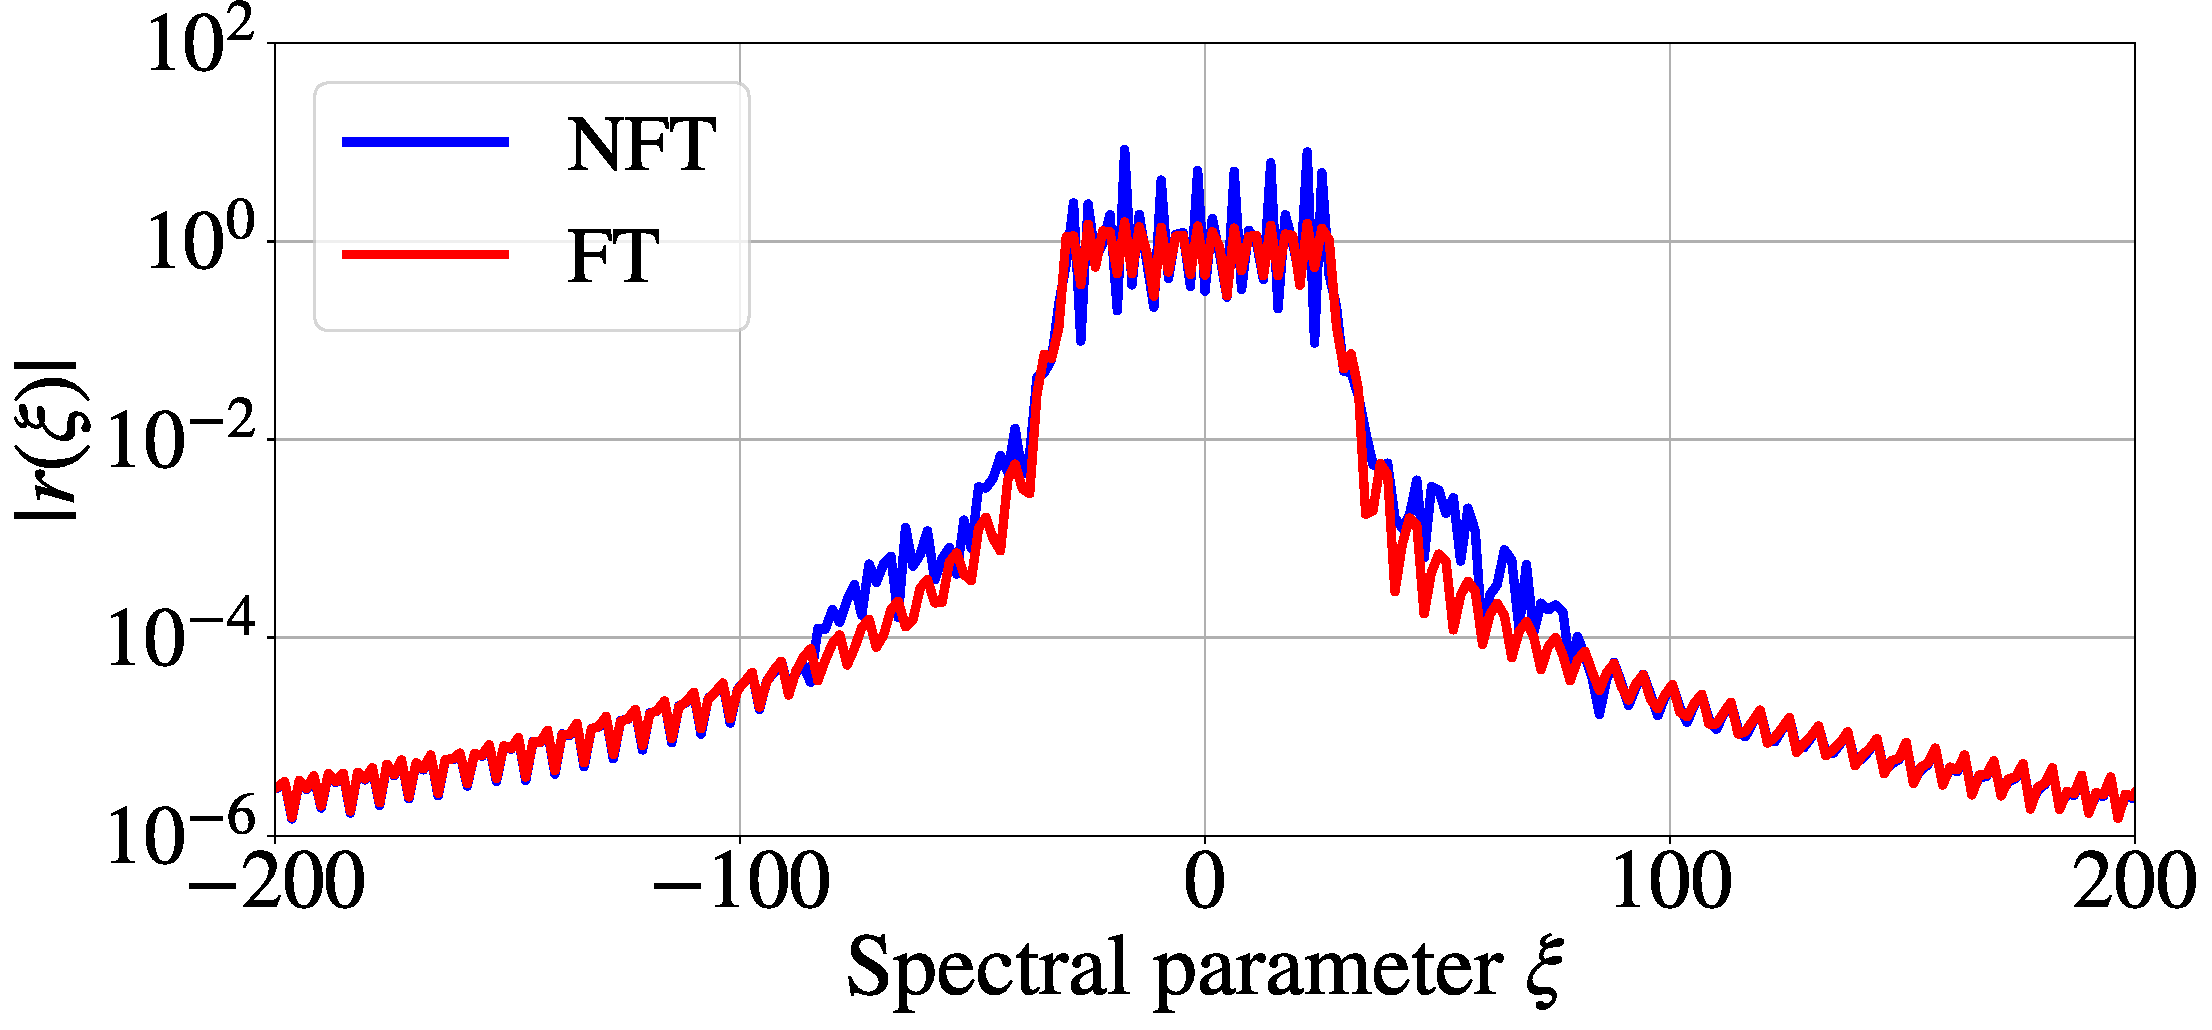
\includegraphics[width=1.\linewidth]{images/nn_nft/scirep_ft_vs_nft_actual.pdf}
\end{minipage}%
\begin{minipage}{.49\textwidth}
  \centering
  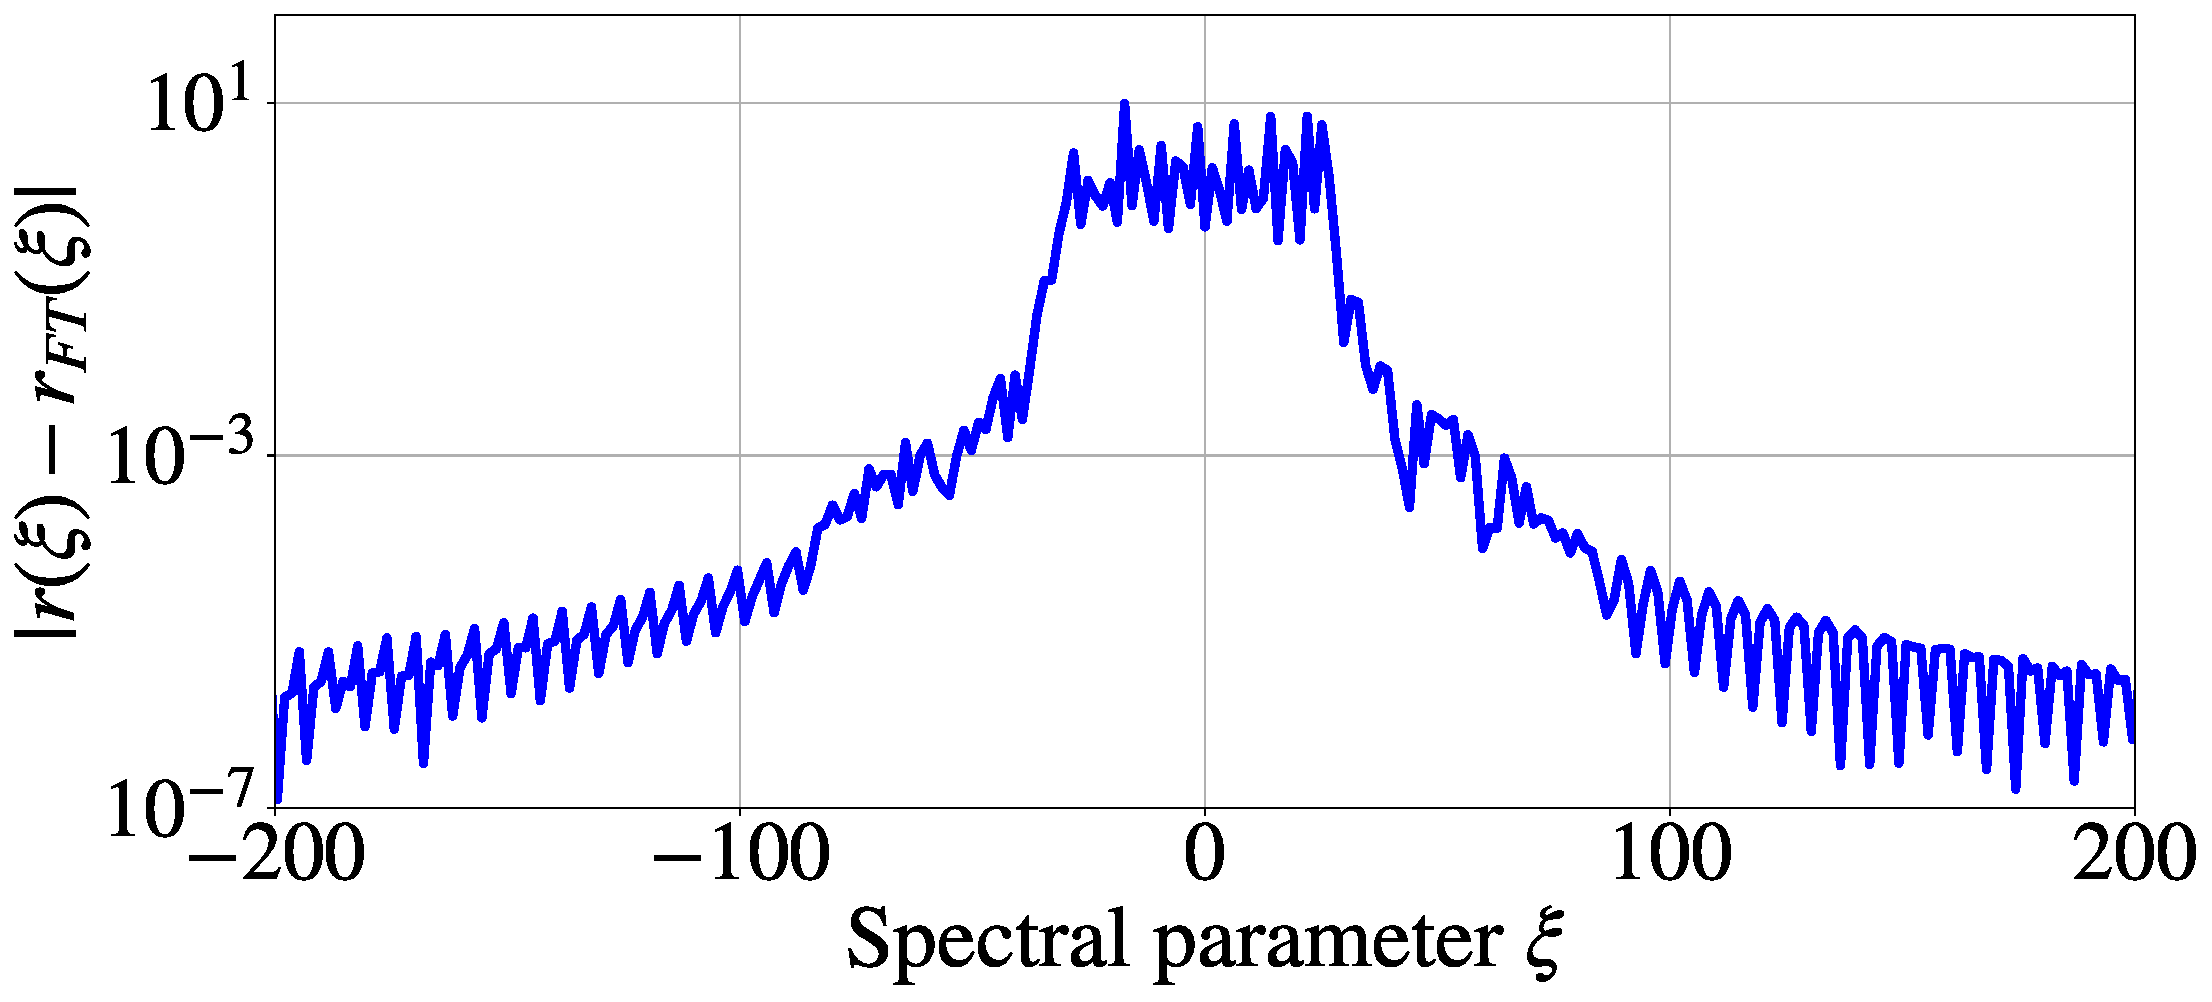
\includegraphics[width=1.\linewidth]{images/nn_nft/scirep_ft_vs_nft.pdf}
\end{minipage}
\caption{\textbf{(a)} Example of the amplitudes of Fourier spectrum (FT) and continuous nonlinear Fourier spectrum (NS) for one of the training signals. \textbf{(b)} Example of the absolute value of the difference between Fourier spectrum and continuous nonlinear Fourier spectrum for one of the training signal. For both graphs signal energy $E_{\text{signal}} = 39.0$ in non-dimensional units.}
\label{fig:nft_and_ft}
\end{figure}

% \subsubsection{Numerical NFT computation}
In our work we used the conventional forward \acrshort{nft} numerical method to generate training and testing data set pairs: the signal and its respective \acrshort{nf} spectrum. %There exists a considerable amount of literature devoted to the different methods for the forward \acrshort{nft} operations \cite{pw18,yk14-2,vps19}.
For the computation of continuous \acrshort{nf} spectrum associated with a given profile $q(t)$ (containing no solitons) having the form of Eq.~(\ref{eq:wdm}), we used the exponential scheme ES4 from the \acrshort{fnft} package\cite{FNFT2018} (non-fast realisation). It has the accuracy proportional to the fourth power of the time sample size, $\sim (\Delta t)^4$. We note that there exists the fast realisation of the \acrshort{nft} processing with $\sim (\Delta t)^4$ accuracy\cite{medvedev2020exponential}, which can potentially be used for efficient NFT-Net training.



\subsection{Neural network design and Bayesian optimisation}


As mentioned above, the general \acrshort{nf} spectrum attributed to a given localised waveform consists of two parts: the discrete spectrum that we do not consider in our current study (our trial pulses do not contain any solitonic component, neither in pure form nor in the noisy case), and the continuous part which is our subject in hand here. The continuous part is retrieved through considering the special Jost solutions (\ref{eq:nlse_jost_matrix}) to the \acrshort{zs} problem (\ref{eq:ZS}). The goal of our work is to demonstrate the fundamental possibility of replacing the direct calculation of \acrshort{nf} spectrum through the numerical solution of the \acrshort{zs} problem (\ref{eq:ZS}) with the computations employing specially-designed and trained \acrshort{nn}s.

The latter task can be addressed using the encoder-decoder approach, where the encoder transforms the input signal into some intermediate vector representation and, later, the decoder converts this representation into the output signal. We notice that the input and output signals can belong to two different data domains. There are several advantages of this approach, e.g. it is quite flexible, so the encoder and decoder structures can differ to match exactly the ``nature'' of each signal's domain. With this, we train such \acrshort{nn}s in the end-to-end style, so the weights of the encoder and decoder will be trained simultaneously and fit each other.
A lot of highly efficient encoder-decoder architectures have been designed up to date, e.g. those can demonstrate an efficiency higher than that of a human brain for some specific tasks \cite{ty2014deepface}. For processing quite long sequences (typically more than 1000 data points), the convolutional \acrshort{nn}s (\acrshort{cnn}) are often more beneficial than the \acrlong{rnn}s (\acrshort{rnn}s). Also, the \acrshort{cnn} allows us to parallelise the computations in an efficient way, which is important in our case. Thus, we argue that the encoder-decoder architectures based on \acrshort{cnn}s are most suitable for our data and task, though other \acrshort{nn} types may also deserve investigation in latter studies.


As a starting point, we took the WaveNet \cite{od2016wavenet}-based network, which extends the concept of deep \acrshort{cnn}s. 
Models of this type have several advantages, among which we underline the reduction of time required for training the network on long data sequences. 
However, a significant drawback of this architecture is the requirement to embed a large number of convolutional layers to increase the receptive field. In our work, to increase the effective size of that region, we used convolutions with dilation. This made it possible to exponentially increase the receptive field with the \acrshort{nn} depth growth and, therefore, to capture a larger number of data points in the input signal. The choice of \acrlong{cnn}s (\acrshort{cnn}s) for \acrfull{nft} applications over simpler neural network architectures is primarily motivated by \acrshort{cnn}s' superior ability to capture spatial hierarchies and complex patterns in data, which are crucial for accurately processing and interpreting signals governed by the nonlinear Schrödinger equation. This inherent capability makes \acrshort{cnn}s particularly well-suited for tasks that require an understanding of the complex, nonlinear dynamics present in \acrshort{nft} analyses.


The momentous issue in using \acrshort{nn}s to perform any nonlinear transformation is the choice of the optimal network architecture. One of the optimisation methods is to enumerate the possible combinations of \acrshort{nn} parameters. But even in the case of a relatively small number of layers, the number of hyperparameters can reach several thousand, which makes the optimisation process very time-consuming, if realisable at all. Thus, the search for an optimisation algorithm for such computationally expensive problems can be extremely difficult. 
Rather than conducting a conventional dimensioning study for \acrshort{nn}s, this research adopts Bayesian Optimization to fine-tune the architecture of the \acrshort{cnn} for the NFT-Net. Bayesian Optimization, recognized for its efficiency in finding the optimal distribution of hyperparameters~\cite{pelikan1999boa}, offers a principled and efficient method for exploring hyperparameter spaces. This approach strikes a balance between model complexity and performance, outperforming exhaustive search methods by utilizing prior evaluations to inform subsequent searches. Through the application of Bayesian Optimization, we systematically refined the \acrshort{cnn} architecture, achieving optimal performance for tasks involving the \acrshort{nft} without resorting to traditional dimensioning studies.
% However, the Bayesian optimisation method~\cite{pelikan1999boa} is deemed to be one of the most efficient optimisation strategies, and so we employ it in this work to find the optimal hyperparameters distribution for the NFT-Net.

% Part about Bayesian 


\begin{figure}[t]
\centering
\begin{minipage}{.49\textwidth}
  \centering
  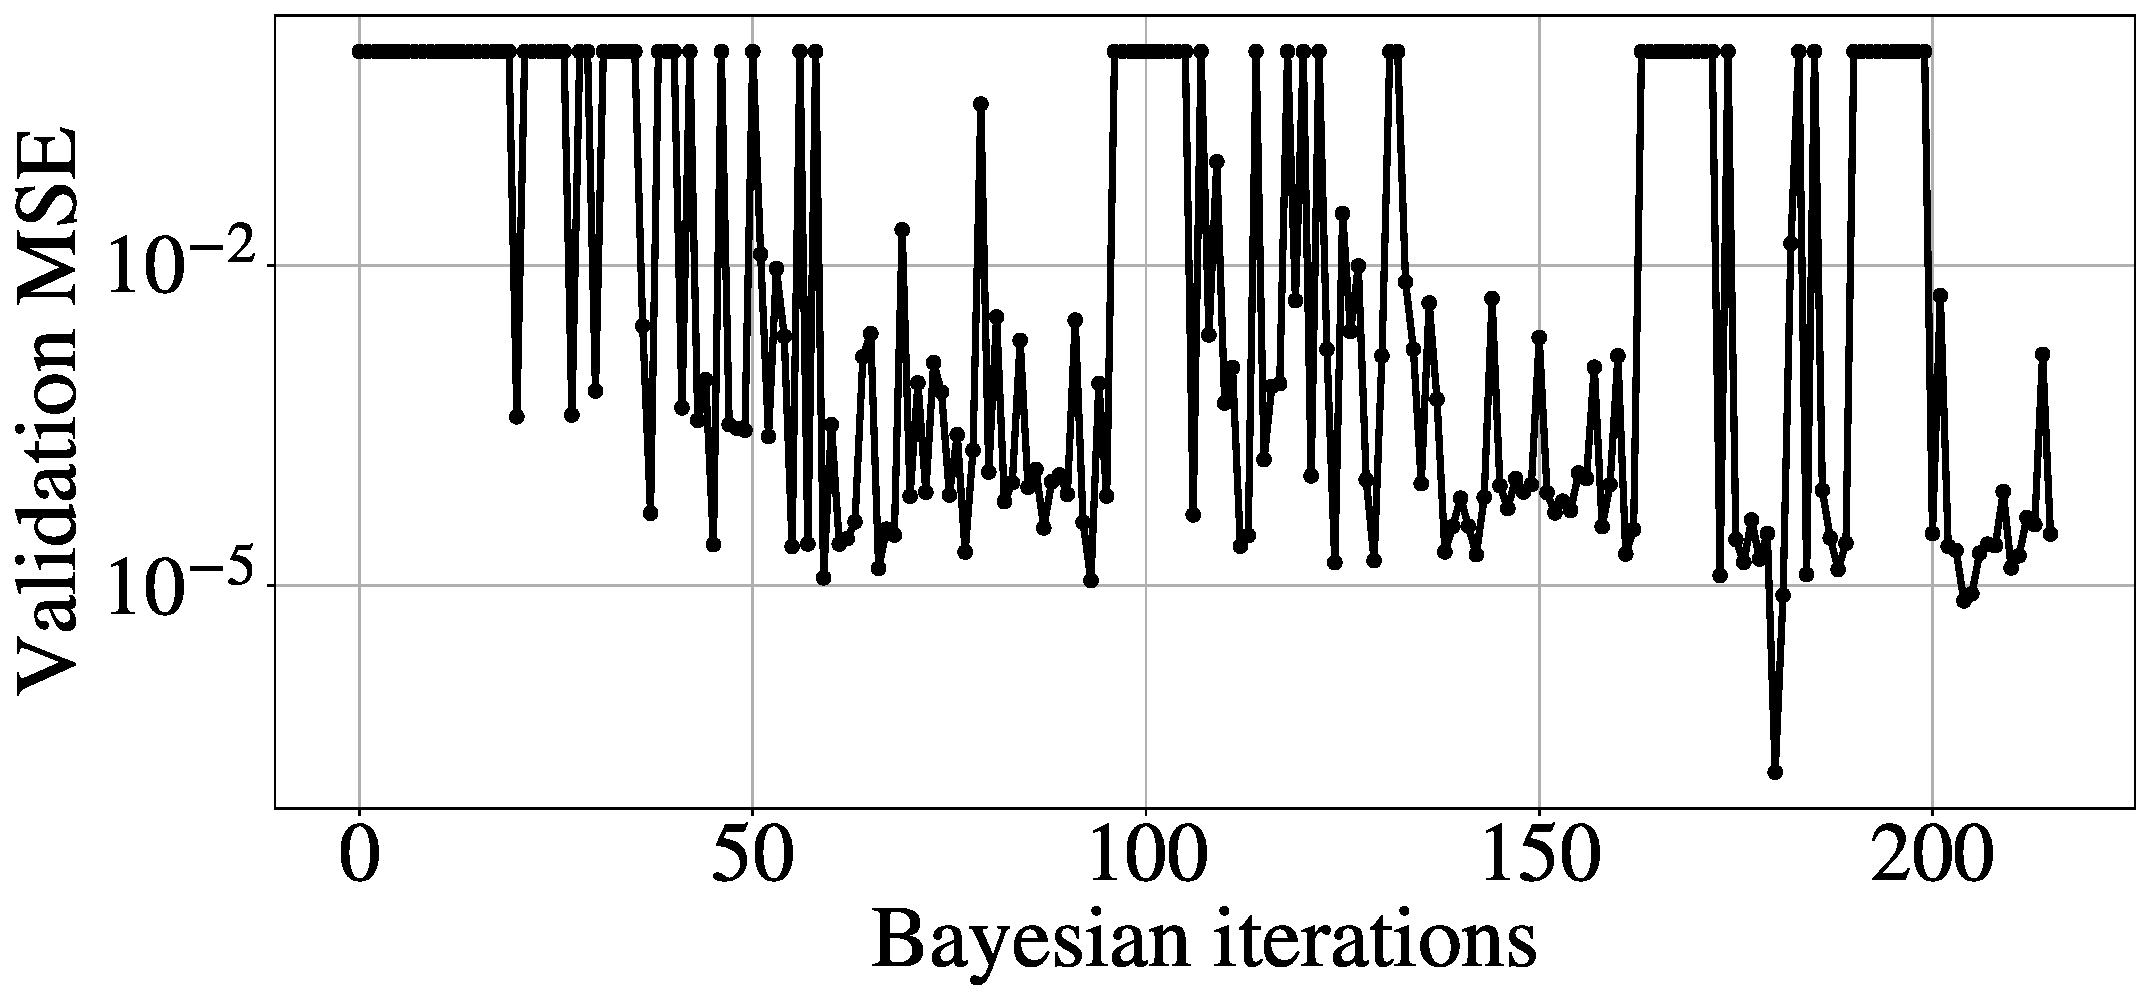
\includegraphics[width=.92\linewidth]{images/nn_nft/scirep_bayes.pdf} (a)
  % \caption{}
  % \label{fig:bayes}
\end{minipage}%
\begin{minipage}{.49\textwidth}
  \centering
  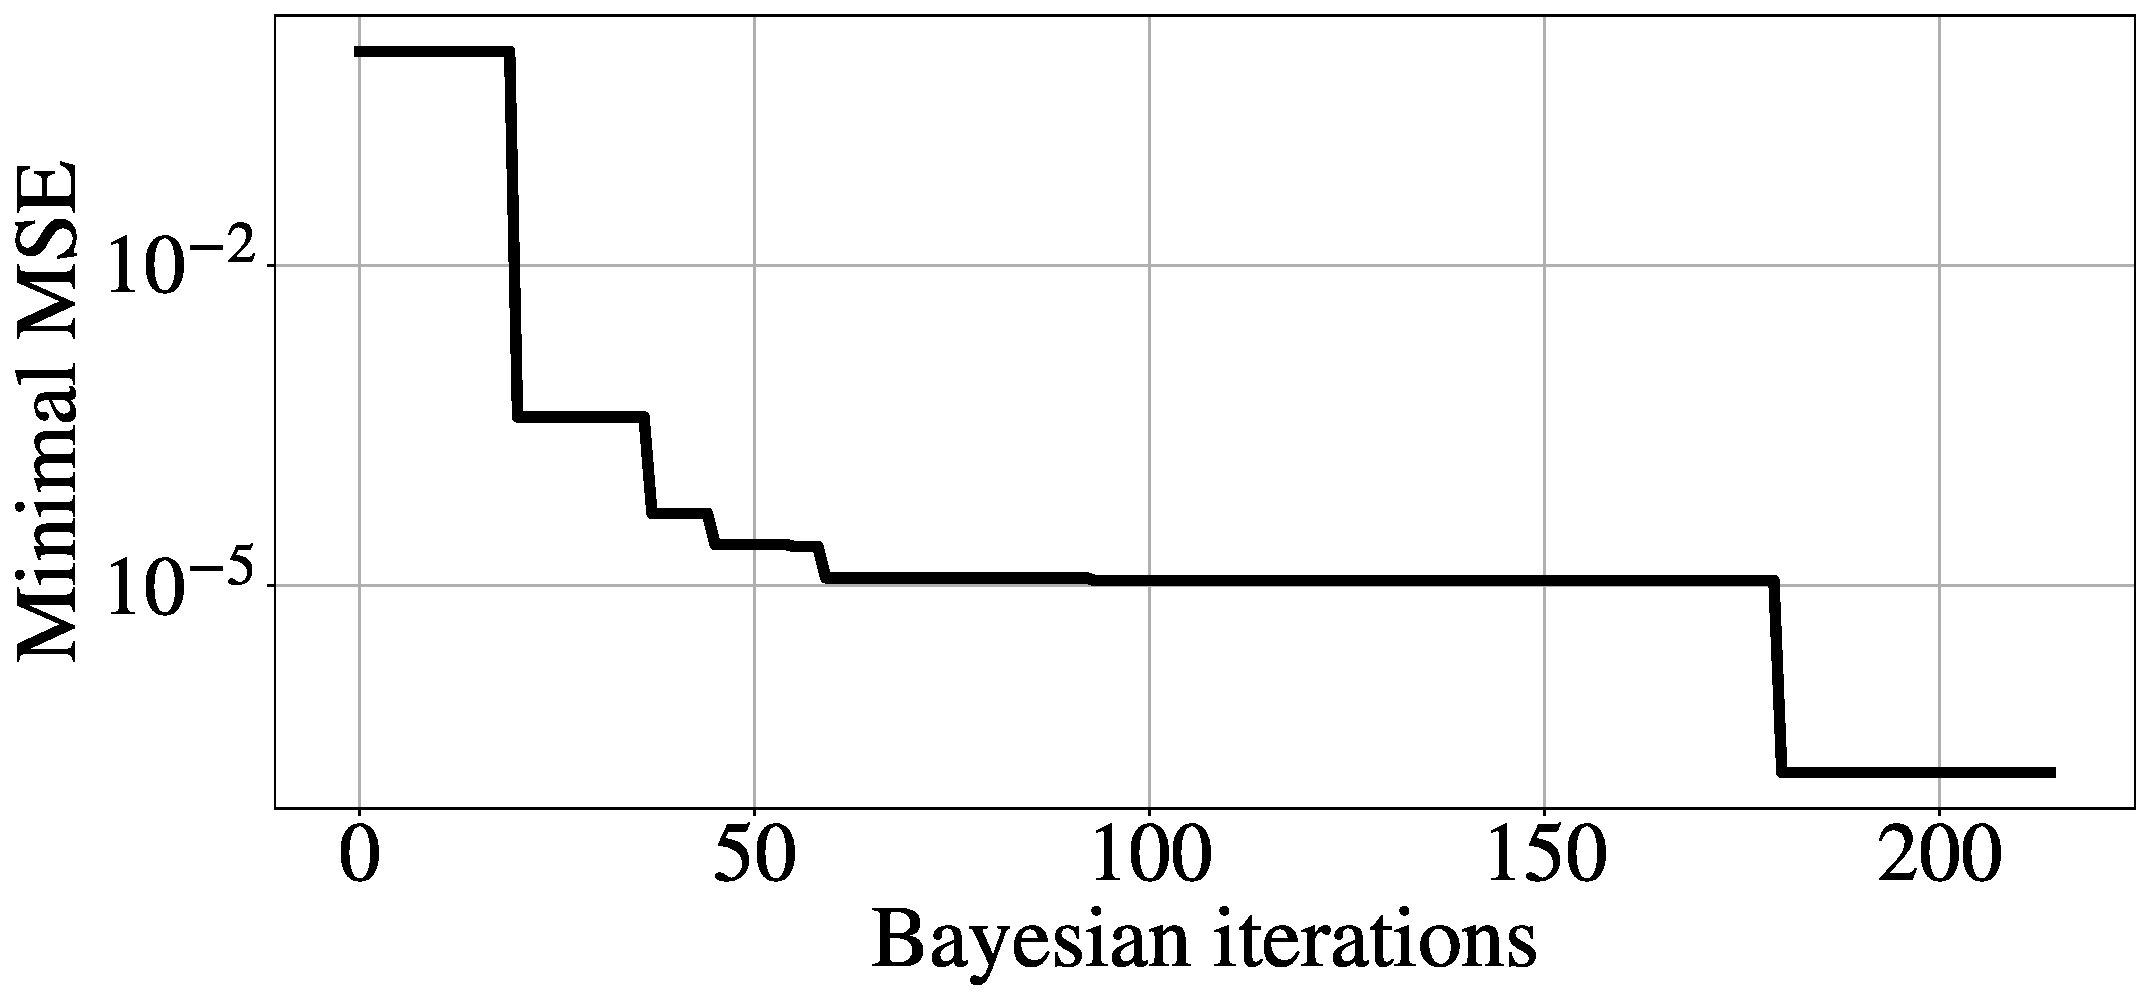
\includegraphics[width=.92\linewidth]{images/nn_nft/scirep_bayes_min.pdf} (b)
  % \caption{}
  % \label{fig:bayes_min}
\end{minipage}
\caption{\textbf{(a)} The dependence of the \acrshort{mse}value on the number of Bayesian iteration. \textbf{(b)} The same for minimal value of \acrshort{mse}.}
\label{fig:bayes_full}
\end{figure}


The Bayesian optimization builds a probabilistic model of the function mapping from hyperparameter values to the objective evaluated on a validation set~\cite{mockus1975bayesian,pelikan1999boa}. By iteratively evaluating a promising hyperparameter configuration based on the current model, and then updating it, the Bayesian optimization aims to gather observations revealing as much information as possible about this function and, in particular, the location of the optimum. Thus, it tries to balance exploration (hyperparameters for which the outcome is most uncertain) and exploitation (the hyperparameters expected to bring us close to the optimum).
An important aspect to note is that the Bayesian optimisation often does not return one specific point in the parameter hyperspace for which the optimised function is minimal. The process converges into some subspace of parameters, where several points can locally minimize the function~\cite{pelikan1999boa}.

\begin{figure}[tbp]
    \centering
    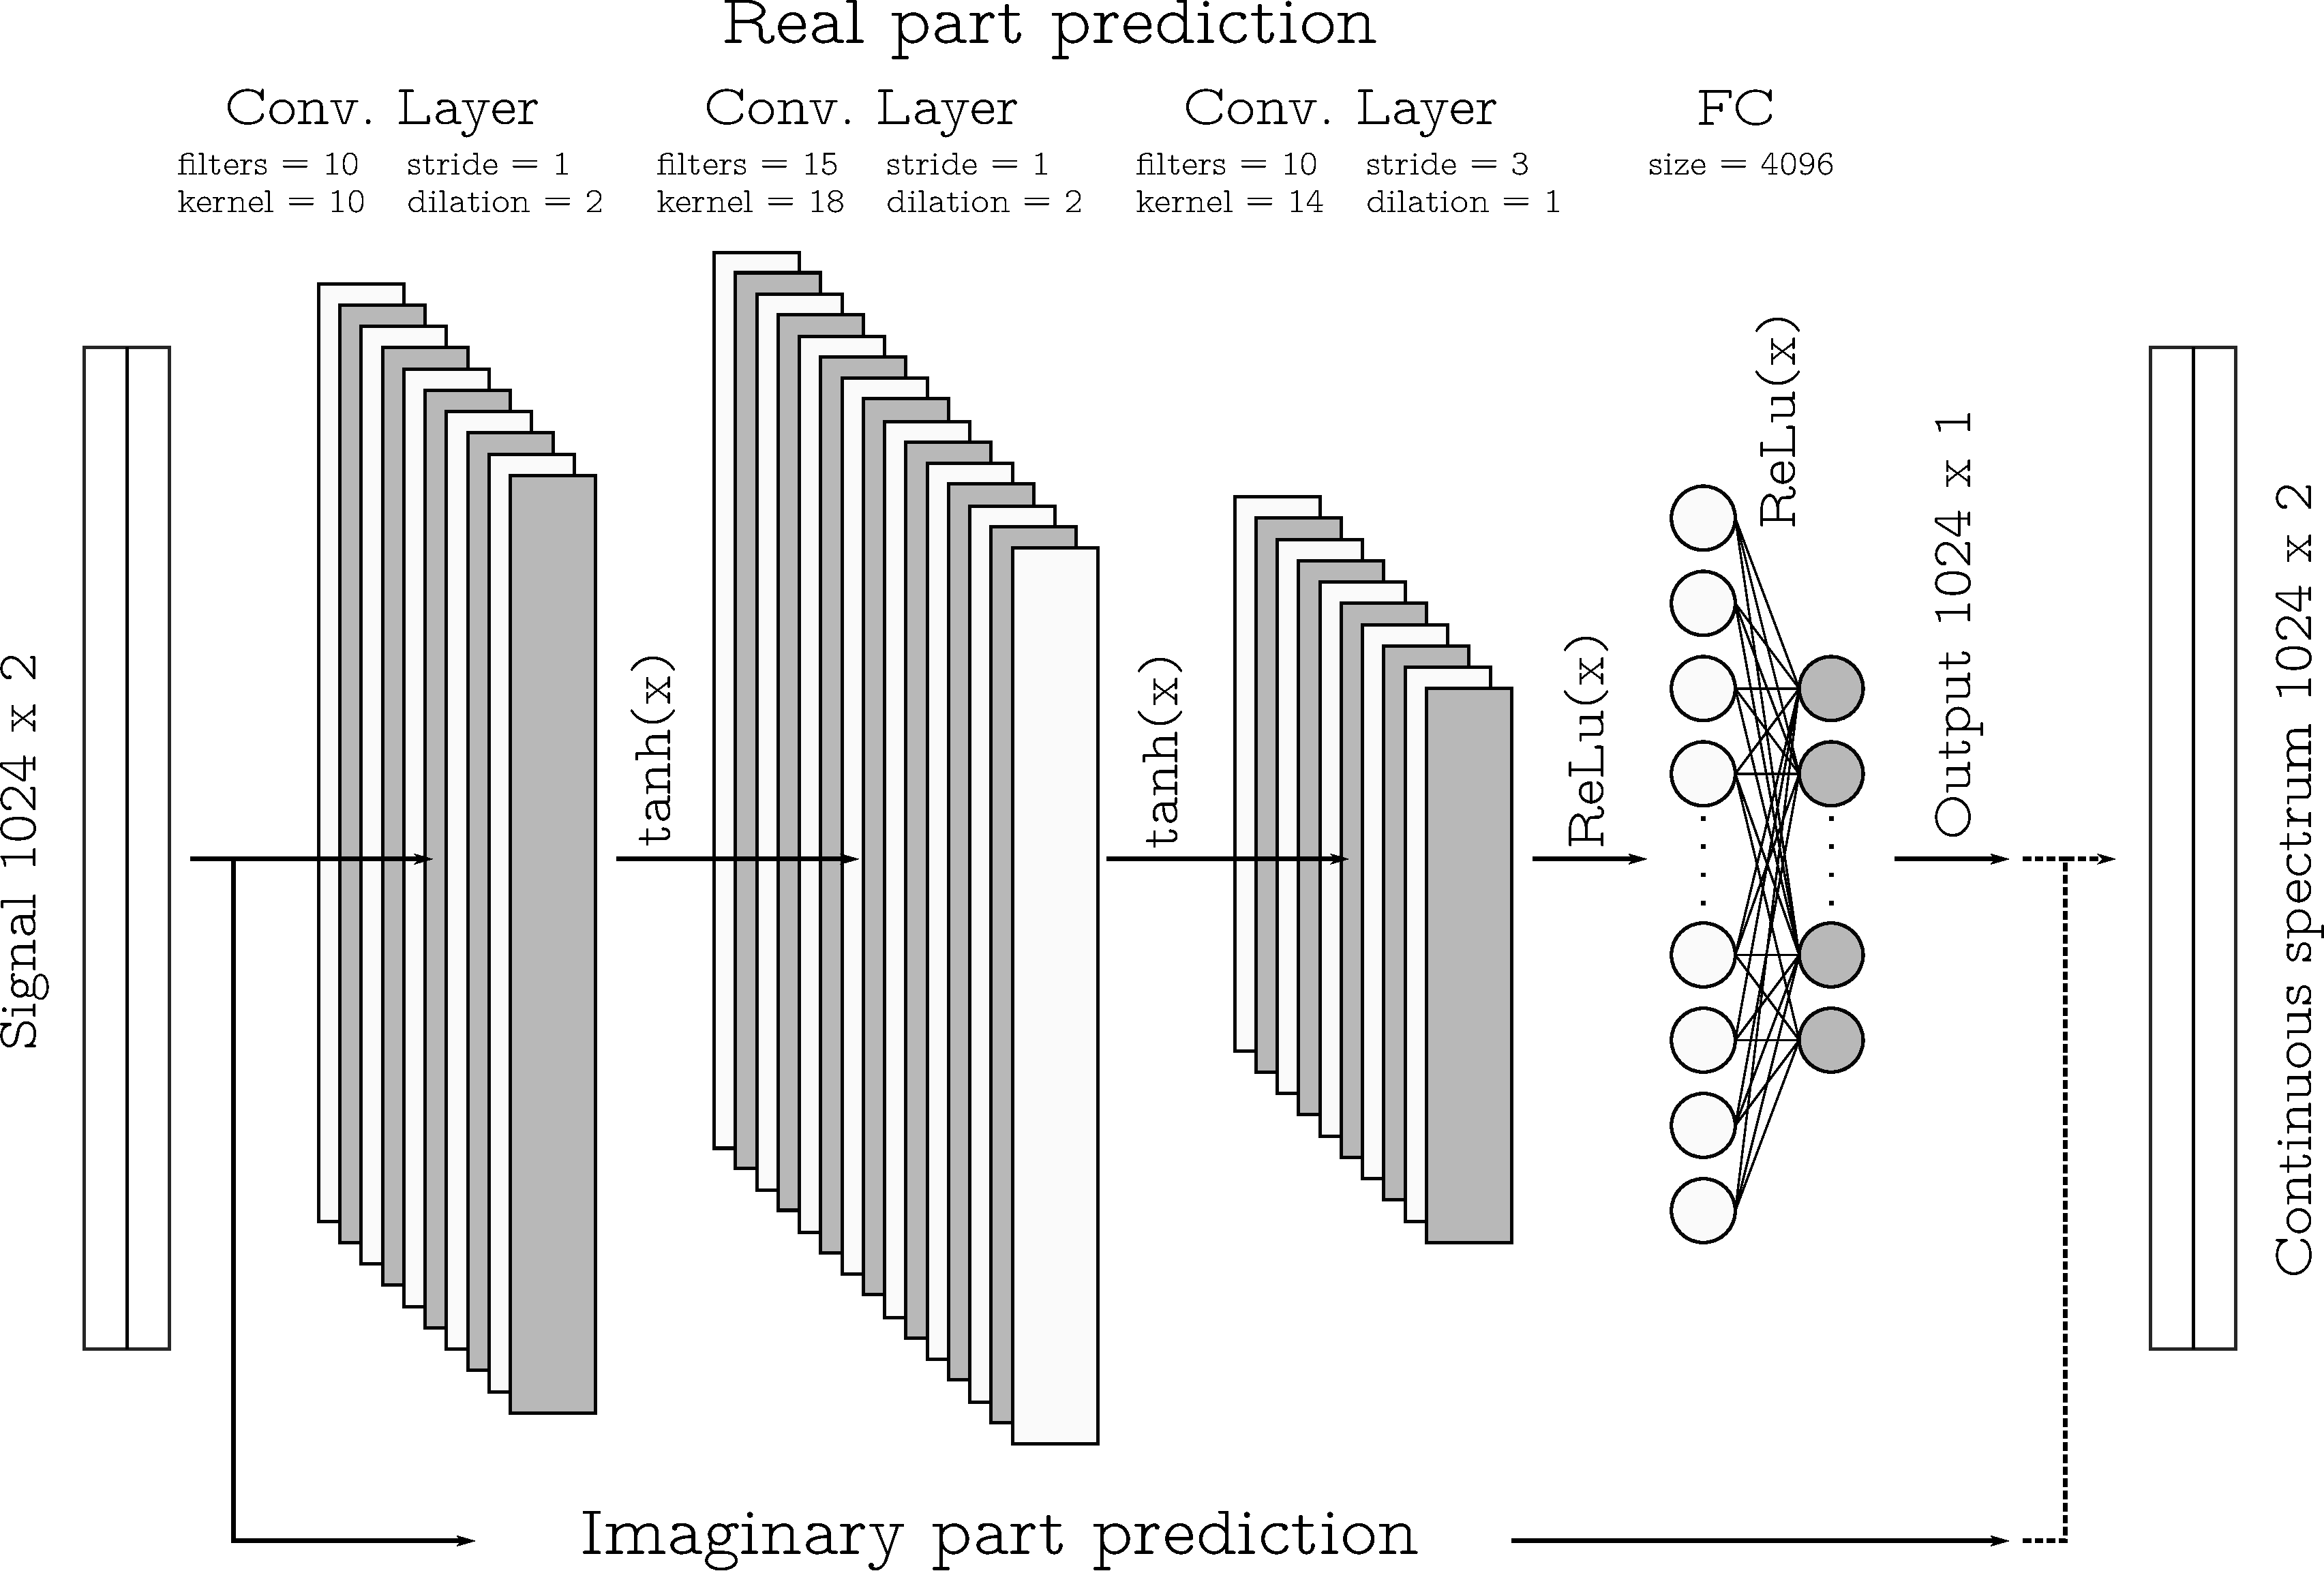
\includegraphics[width=1.0\linewidth]{images/nn_nft/arch_new.pdf}
    \caption{The schematic of NFT-Net topology: the extended scheme presents the sequence of operations for the processing of real part; the processing of imaginary part is identical (marked with the long arrow below the scheme). The numbers indicating the layers/arrays sizes refer to our processing 1024 complex-valued signal samples.}
    \label{fig:nn_architecture}
\end{figure}

% Part about how we did it

We manipulate the following hyperparameters for the convolutional part of the neural network: the number of convolutional layers, the number of filters, the kernel size, stride, dilation, and the activation function for each layer. After the convolutional part, there are 2 fully connected layers, the second of which has a fixed size (1024, which corresponds to the size of the output vector). The size and activation function of the first fully connected layer was also a hyperparameter for optimization.
The optimization process included fine-tuning the number of convolutional layers within a range of 2 to 4, allowing for variability in the depth of feature extraction. For each convolutional layer, the number of filters was set to span between 10 to 256, depending on the layer, to diversify the capacity for feature detection. The kernel size, crucial for defining the scope of input considered at each convolutional step, varied from $1 \times 1$ to $20 \times 20$, offering flexibility in the granularity of analysis. Stride and dilation parameters, both adjustable from 1 to 3, were optimized to alter the convolution operation's coverage and input sampling methodology, respectively. The architecture also incorporated 1 to 3 dense layers, with the neuron count in each layer ranging broadly from 128 to 4096, providing a robust framework for pattern recognition and decision-making. Activation functions -- ReLU, sigmoid, and tanh -- were selectively employed across the network to introduce nonlinearity, enhancing the model's ability to model complex relationships in the data. This comprehensive and detailed parameterization ensures a thorough exploration of the model's architectural landscape, aiming to identify configurations that yield optimal performance metrics. In each iteration of Bayesian optimization, we retrain the \acrshort{nn} and calculate the \acrshort{mse}loss on the validation dataset. The architecture of the \acrshort{nn} is considered better if it results in a lower validation loss. Therefore, we select the architecture that achieves the lowest loss value on the validation dataset.

For the optimisation, we used a dataset without additional noise and employed only the real part of the continuous spectrum for the prediction. After that, the ``optimal'' architecture (but not weights) is fixed, and is no longer changed to predict the imaginary part of the continuous spectrum or for our operating with the datasets with additional noise.
The loss function was optimised for each architecture. We used the \acrshort{mse}as the loss function, aiming to minimise the \acrshort{mse} between the network output and the target output computed with the conventional \acrshort{nft} method~\cite{FNFT2018}. In training, we employed the Adam (Adaptive Moment Estimation) optimisation algorithm with the learning rate of 1e-4 ~\cite{s2000adaptive}. 
The learning process of each point in the parameter hyperspace was stopped if the value of the loss function did not decrease over 5000 epochs. 
We chose this large epoch stopping-criterium number to neutralise the factor of randomness in the learning process, which appears due to the random choice of the initial weights. Additionally, we checked the value of the loss function on the validation set to prevent the overfitting, but for the amount of training data used, the overfitting was not observed. 
Figure~\ref{fig:bayes_full} presents the dependence of the \acrshort{mse} value and dependence of its minimum on the  Bayesian iteration number. For architectures with more than 20 million training parameters, we set the value of the loss function to $1.0$: this explains the upper cut-off limit in the figure. It is apparent from Fig.~\ref{fig:bayes_full} that the optimisation has identified a subspace where many architectures have approximately the same value of the loss function at the level of $10^{-5}$. However, there was a point where the value was at the level of $10^{-7}$. Thus, we took this point (a set of hyperparameters) as the optimal one.
After finding the optimal architecture, each \acrshort{nn}'s weights were trained for different \acrshort{snr} but keeping the same optimal architecture parameters. On average, with the amount of data used, our learning process took 50 000 epochs to reach the minimum for each noise level.

% End of the optimisation part

The original signal and \acrshort{nf} data for the continuous spectrum are complex-valued functions. Therefore, two networks with the same architecture are to be used for the whole transformation; each identical part is responsible for the computation of either the real or imaginary parts of the resulting arrays, which contain the values of continuous \acrshort{nf} spectrum defined in~Eq.~(\ref{eq:nlse_r}).  Fig.~\ref{fig:nn_architecture} depicts the schematic for the entire optimised NFT-Net architecture. The convolutional part consists of three layers with 10, 15 and 10 filters. Kernel sizes of the first and third convolutional layers are 10, and for the layer between them, it is 18. As noted above, we took the dilation value for each layer as one of the sought hyperparameters. For NFT-Net, the optimisation gave that the first two layers have dilation 2, stride 1 and ``tanh'' activation function, and for the third layer, the dilation is 1 with stride 3 and ``ReLu''  activation. After the \acrshort{cnn} part we put the flattening layer, not shown in the figure (but affecting the processing complexity), and two fully-connected layers with 4096 and 1024 neurons. The exemplary picture of how the designed \acrshort{nn} works on one signal is given in Fig.~\ref{fig:wdm_and_spectrum}. In this figure, we show the results of the \acrshort{nn}-based \acrshort{nf} spectrum computation for the noiseless case. Already from this figure, we can notice that the result produced by our \acrshort{nn} and that obtained from conventional \acrshort{nft} routine\cite{FNFT2018} are very similar. 


\subsection{Studying the NFT-Net performance for computing \acrshort{nf} spectra of noisy signals}

In this section we analyse the NFT-Net performance and the denoising property of the \acrshort{nn}. We compare the deviations in the obtained nonlinear spectrum calculated with the NFT-Net and calculated with the conventional \acrshort{nft} applied to the same signal without noise. To quantify the performance rendered by the NFT-Net application with the performance of conventional algorithms applied to noisy signals, we use the following metric:
\begin{equation}
    \eta = \frac{1}{S} \, \sum_{i = 1}^{S} \langle \eta_i(\xi) \rangle_{\xi},
    \quad
    \eta_i(\xi) = \frac{|\{r_\text{predicted}(\xi)\}_i - \{r_\text{actual}(\xi)\}_i| }{\langle |\{r_\text{actual}(\xi)\}_i| \rangle_{\xi}} {,}
    \label{eq:metric}
\end{equation}
where $S$ is the total number of signals in the validation set, $\langle \cdot \rangle_{\xi}$ denotes the mean over the spectral interval, 
$\{r_{\text{predicted}}(\xi)\}_{i}$ and $\{r_{\text{actual}}(\xi)\}_{i}$ correspond to the value of reflection coefficient $r(\xi)$ computed for the signal number $i$ at point $\xi$ (we compare the quantities for the validation data set).  The label ``predicted'' refers to the result produced by the NFT-Net on the noisy signal, and ``actual'' marks the $r(\xi)$ value obtained using the conventional \acrshort{nft} algorithm\cite{FNFT2018} for the noiseless signal.
The relative error $\eta(\xi)$ is determined at the point $\xi$, so we use $\langle \eta(\xi) \rangle_{\xi}$ to estimate the overall mean of the error for one signal, and use Eq.~(\ref{eq:metric})  to evaluate the error for the entire validation dataset.
We stress that the metric was chosen in such a way as to take into account even the regions where the value of the spectrum is much less than one.


\begin{figure}[htbp]
\centering
\begin{minipage}{.47\textwidth}
  \centering
  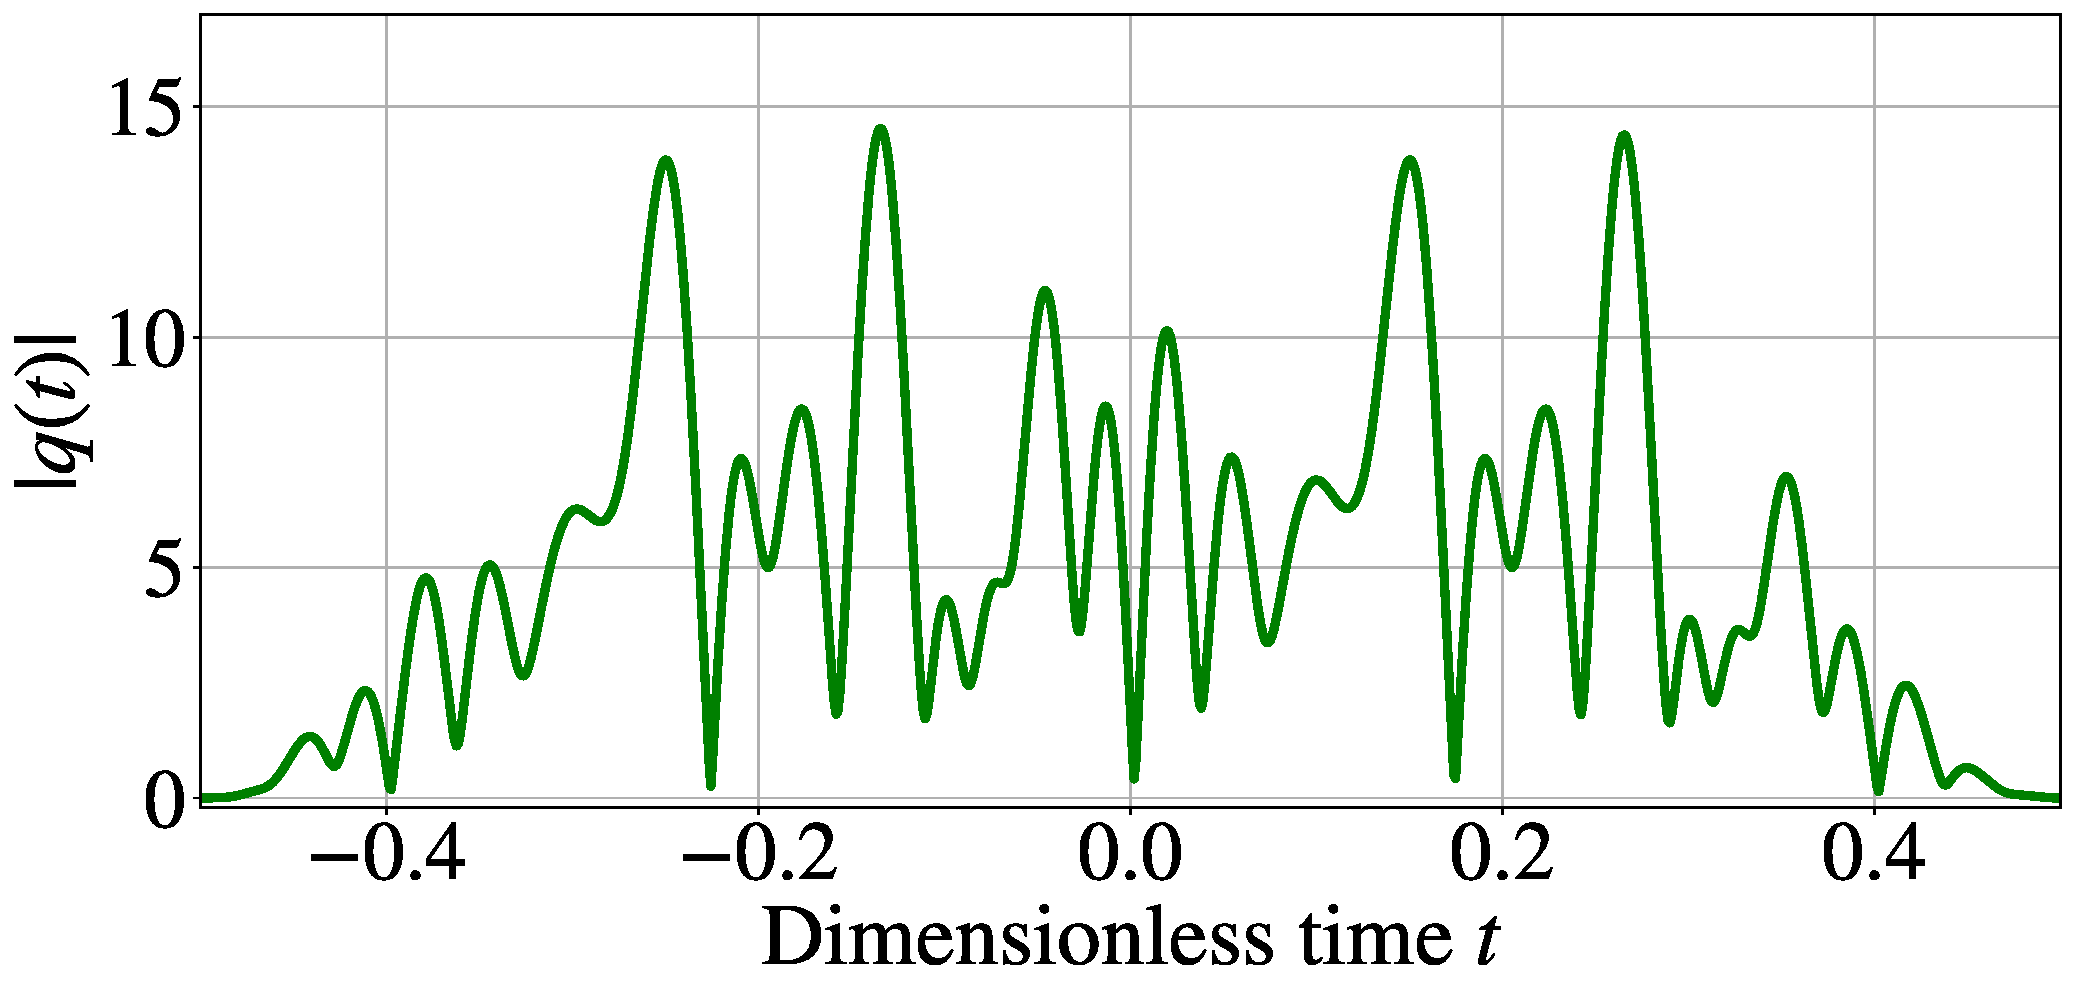
\includegraphics[width=1.\linewidth]{images/nn_nft/scirep_signal_example.pdf}
  \center{(a) Amplitude of original signal}
  % \label{fig:won_signal}
\end{minipage}%
\hfill
\begin{minipage}{.47\textwidth}
  \centering
  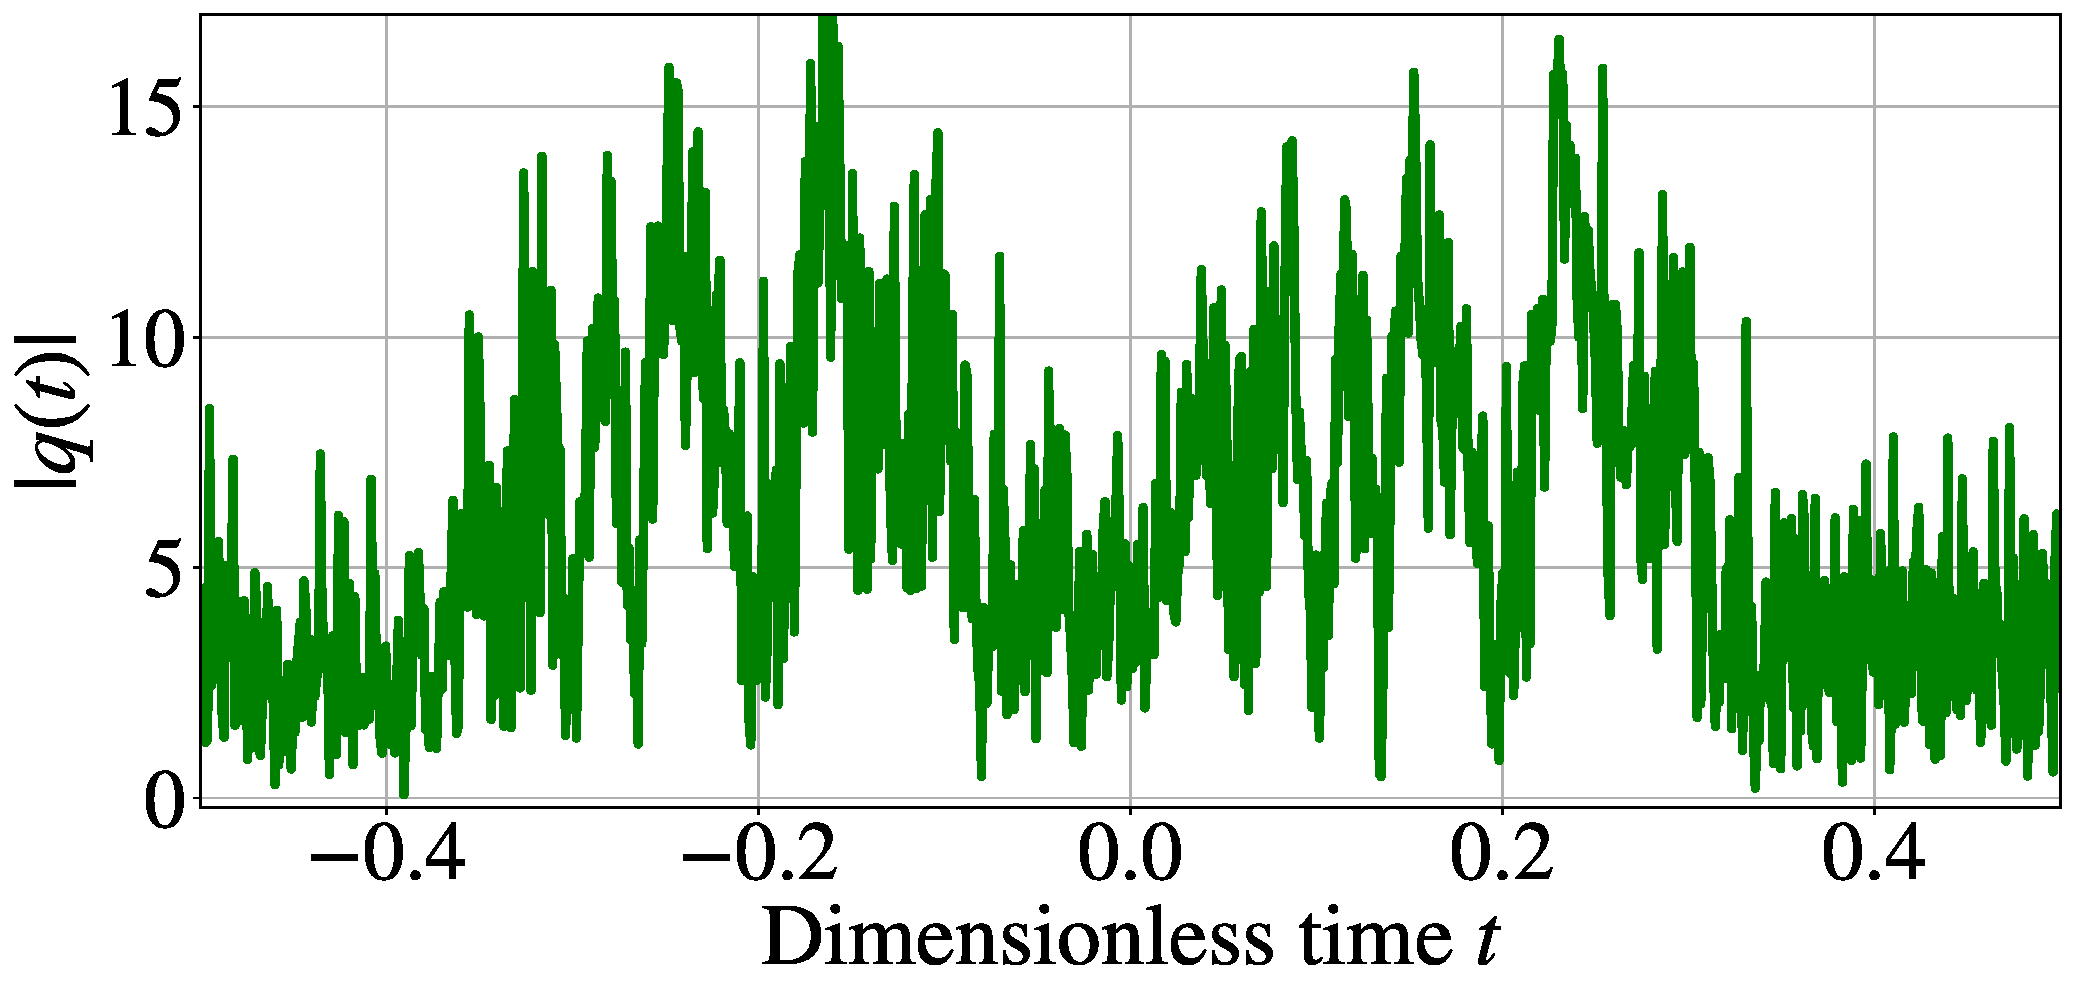
\includegraphics[width=1.\linewidth]{images/nn_nft/scirep_signal_wn_example.pdf}
  \center{(b) Amplitude of signal with additional noise}
  % \label{fig:wn_signal}
\end{minipage}
\\

\begin{minipage}{.47\textwidth}
  \centering
  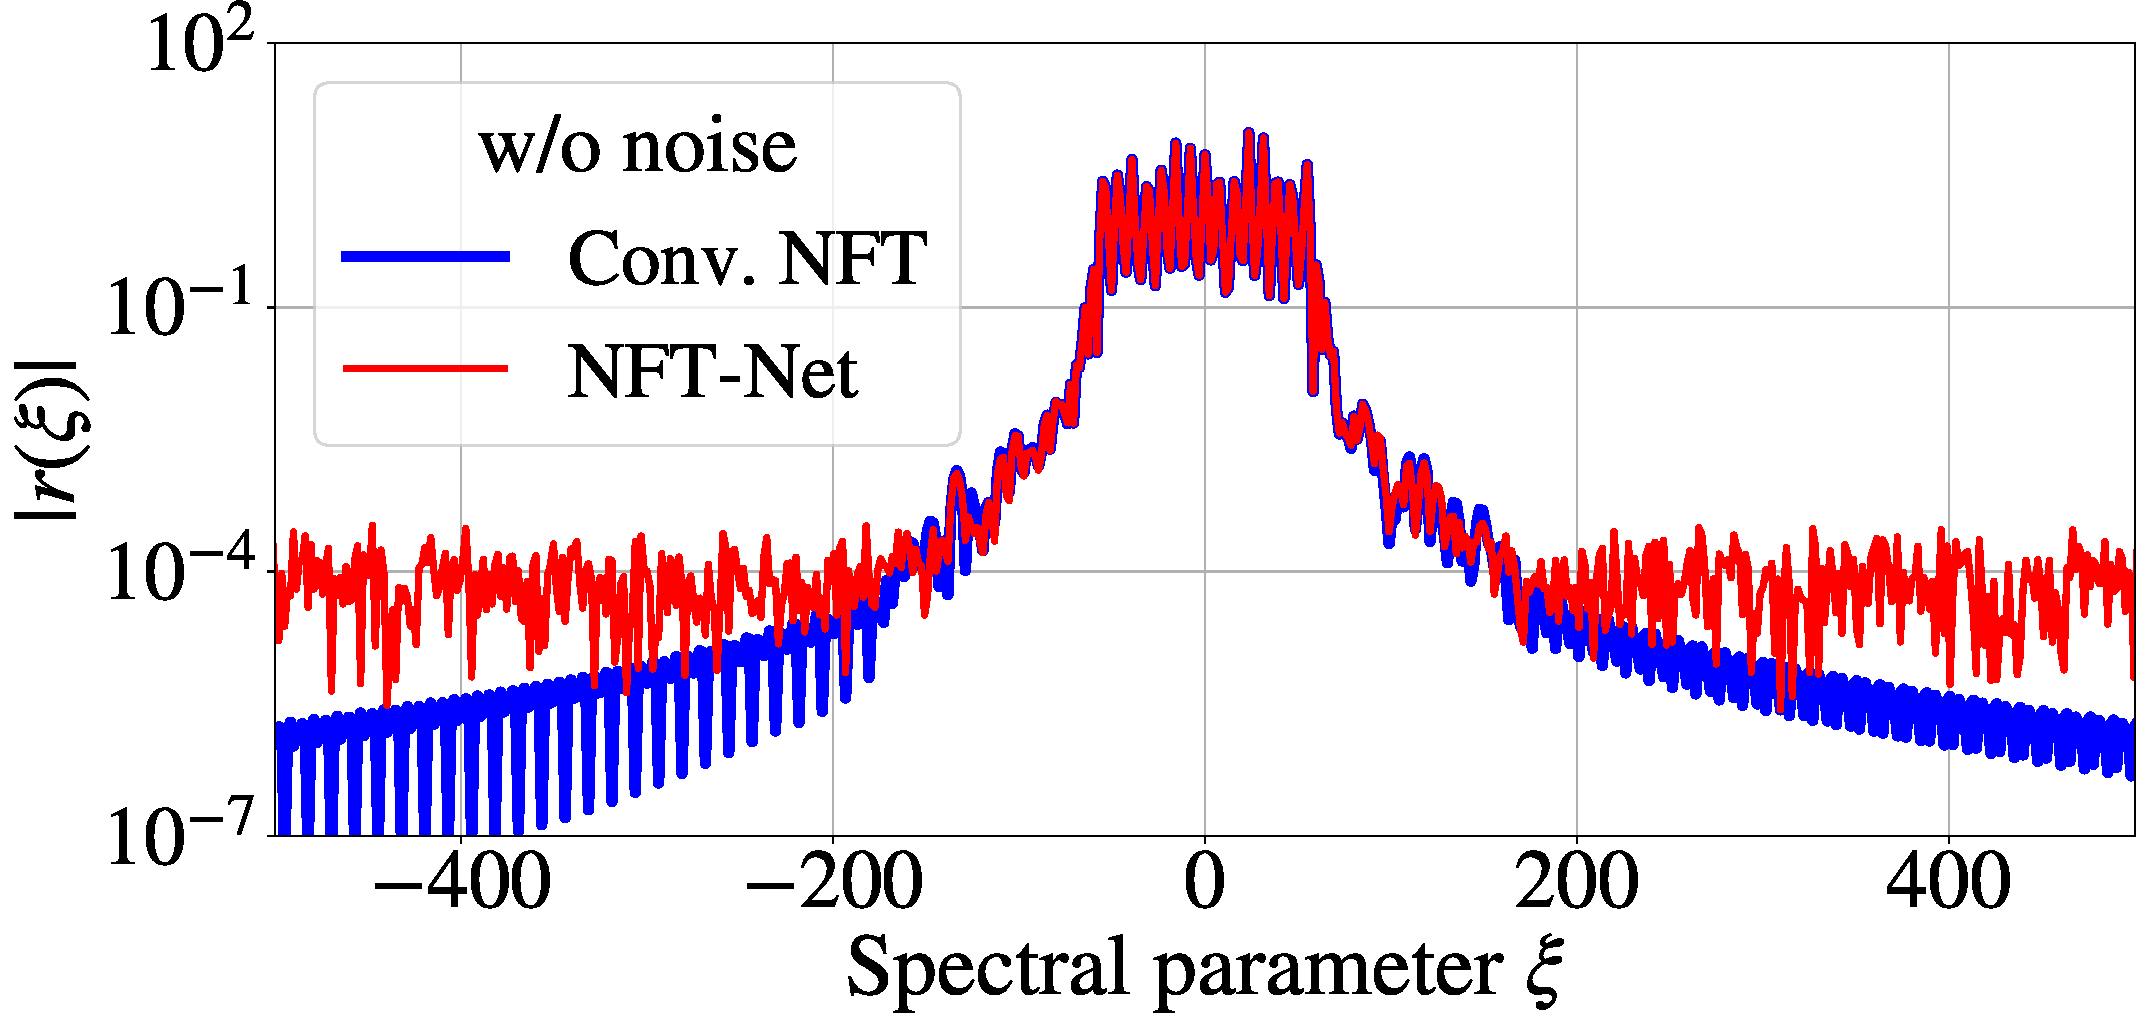
\includegraphics[width=1.\linewidth]{images/nn_nft/scirep_cont_spec_example.pdf}
  \center{(c) Amplitude of reflection coefficient for continuous spectrum}
  % \label{fig:won_spectrum}
\end{minipage}
\hfill
\begin{minipage}{.47\textwidth}
  \centering
  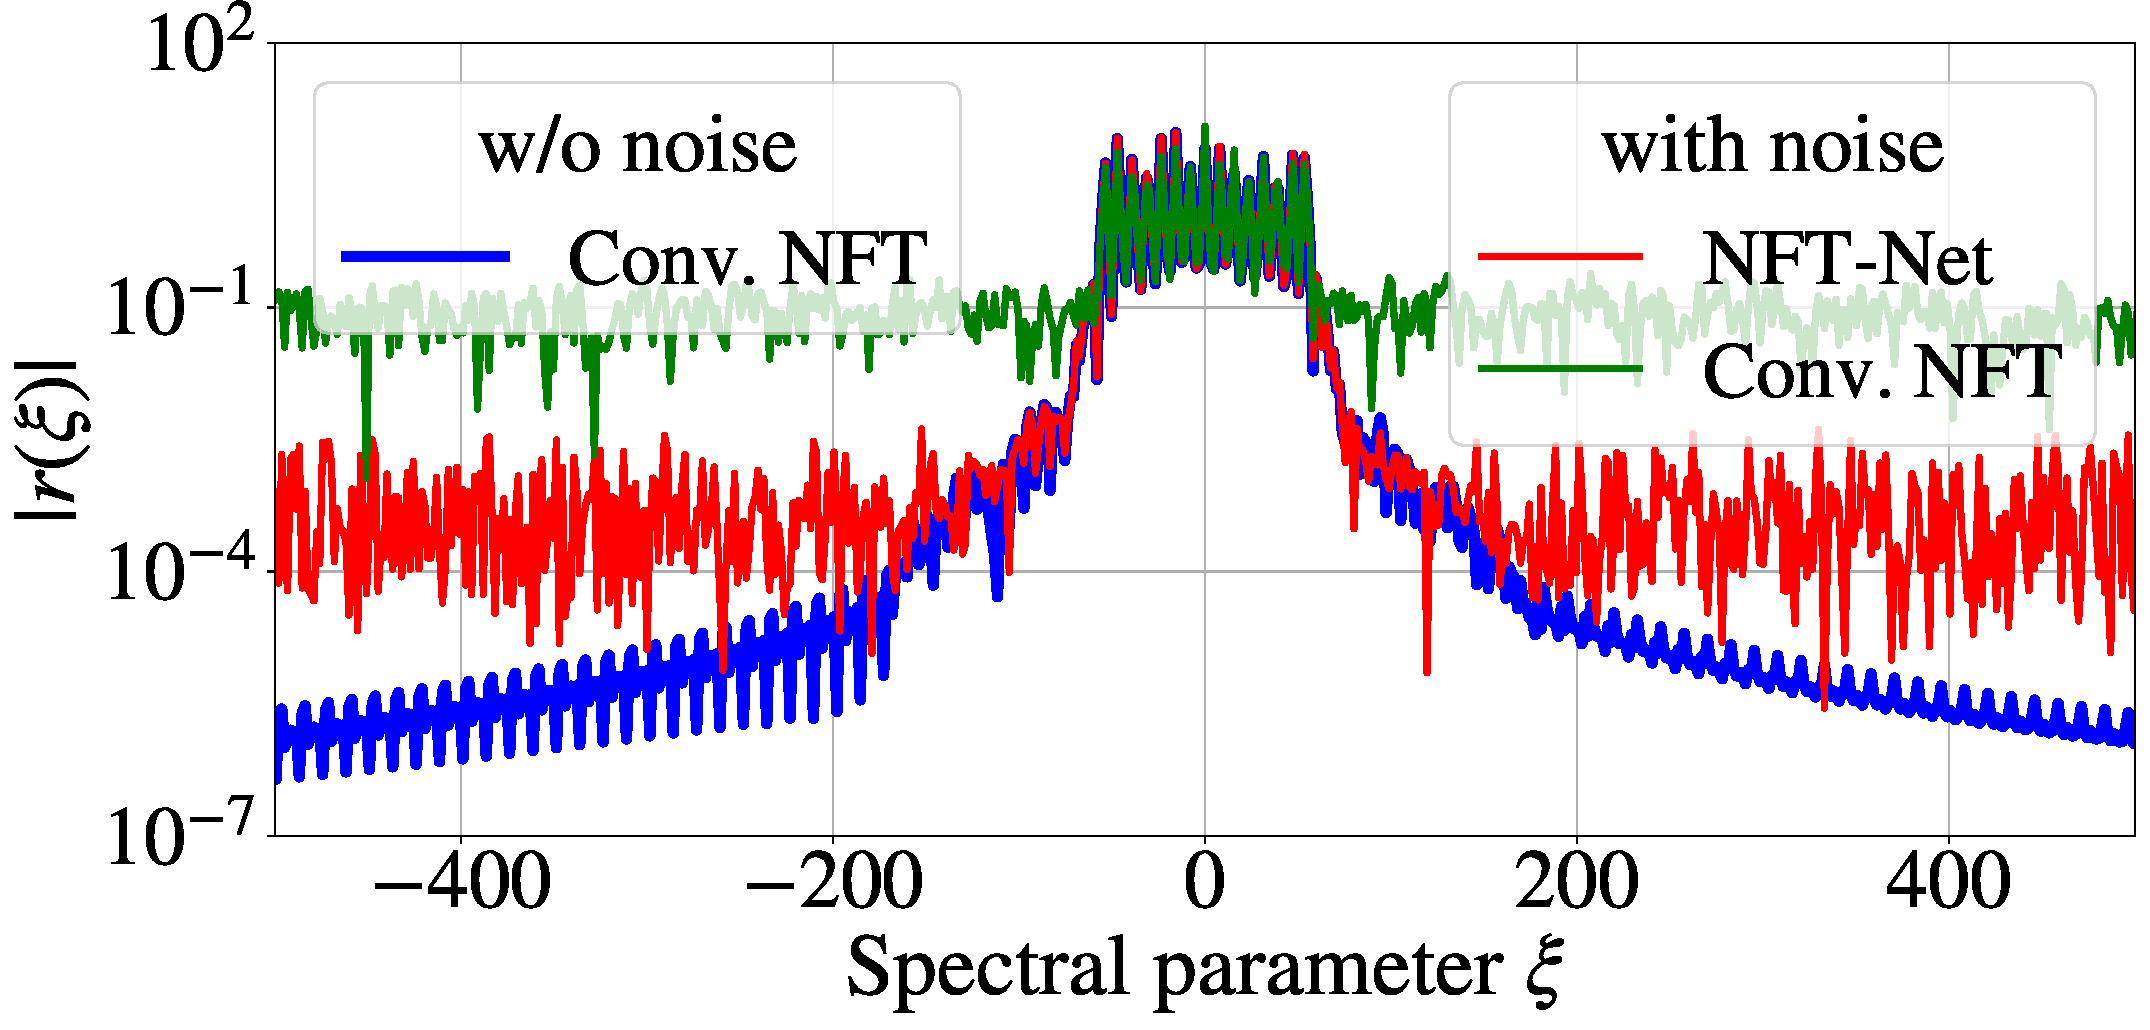
\includegraphics[width=1.\linewidth]{images/nn_nft/scirep_cont_spec_wn_example.pdf}
  \center{(d) Amplitude of reflection coefficient for continuous spectrum}
  % \label{fig:wn_spectrum}
\end{minipage}
\\

\begin{minipage}{.47\textwidth}
  \centering
  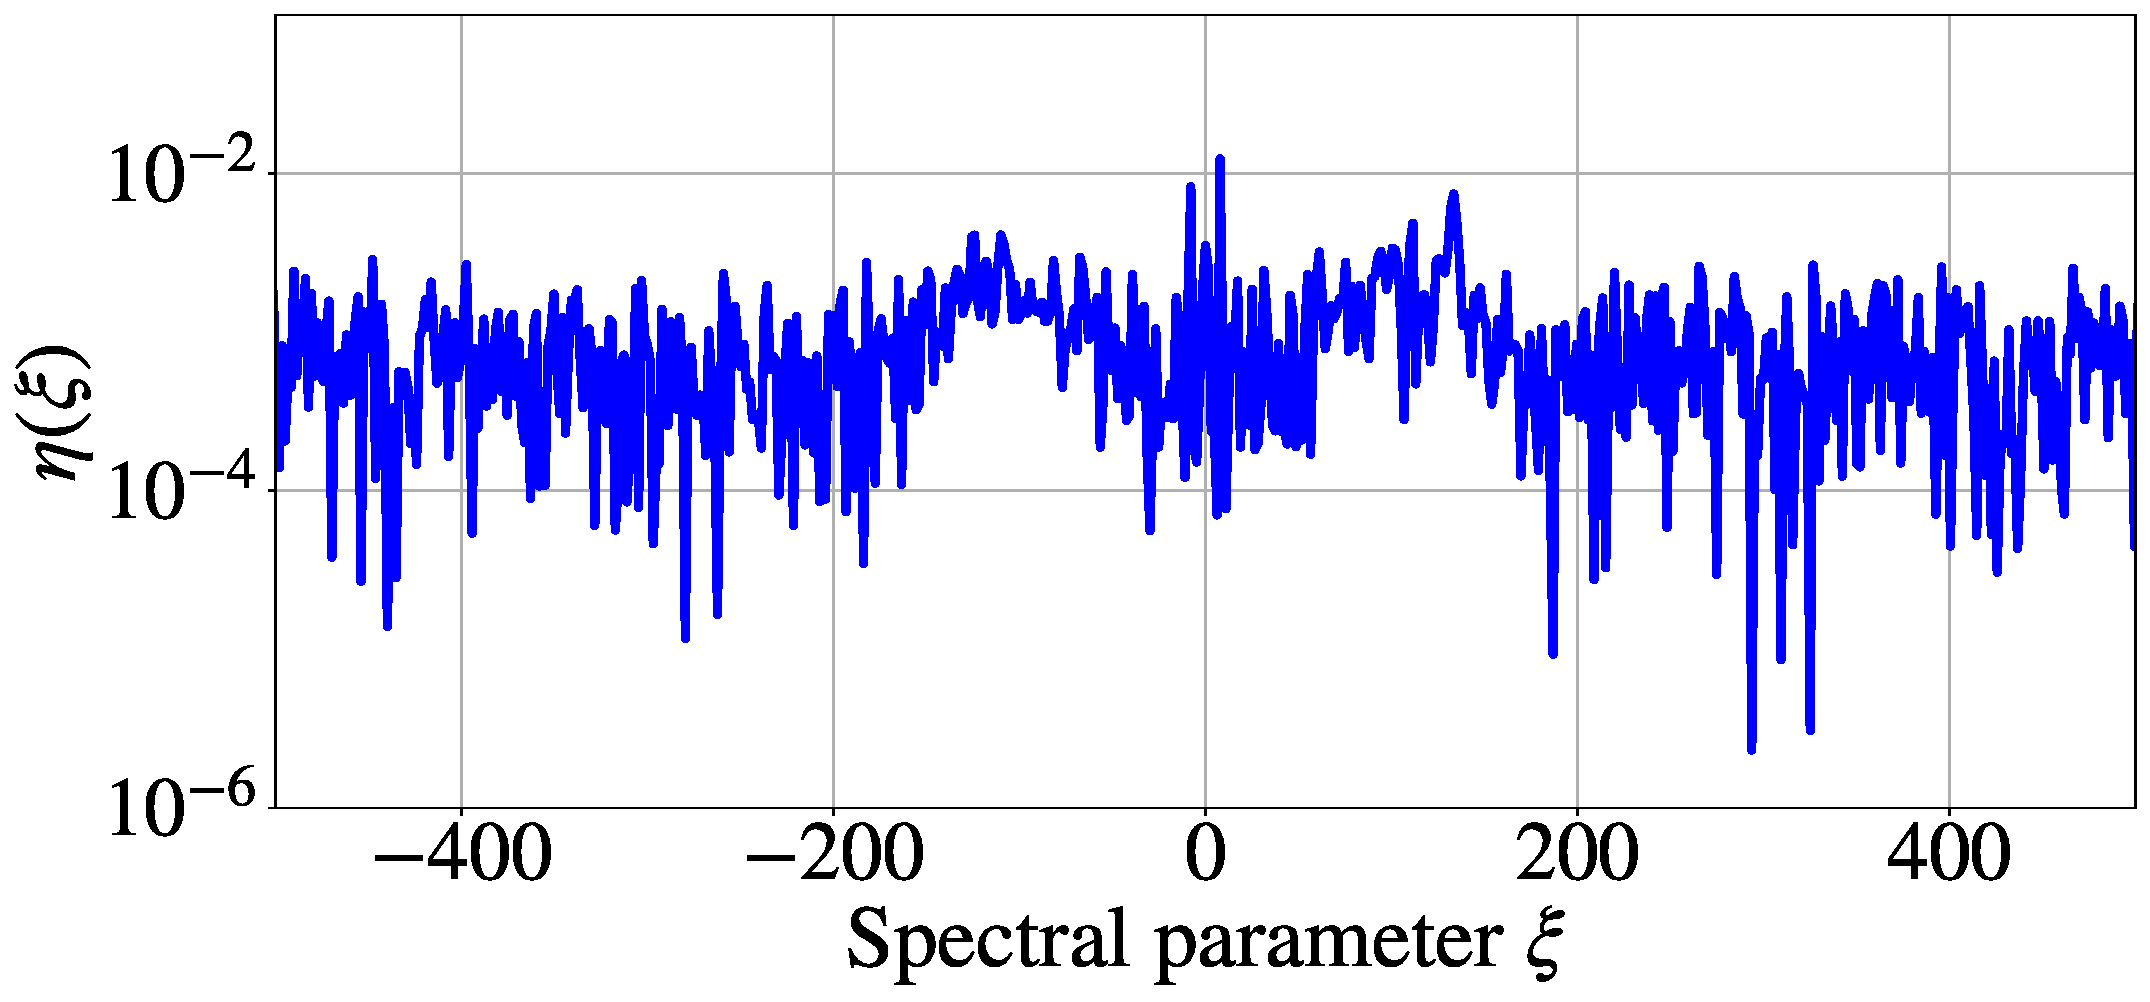
\includegraphics[width=1.\linewidth]{images/nn_nft/scirep_spectrum_diff_example.pdf}
  \center{(e) Difference between $r(\xi)$ calculated using NFT-Net and Conv. \acrshort{nft}}
  % \label{fig:won_diff}
\end{minipage}
\hfill
\begin{minipage}{.47\textwidth}
  \centering
  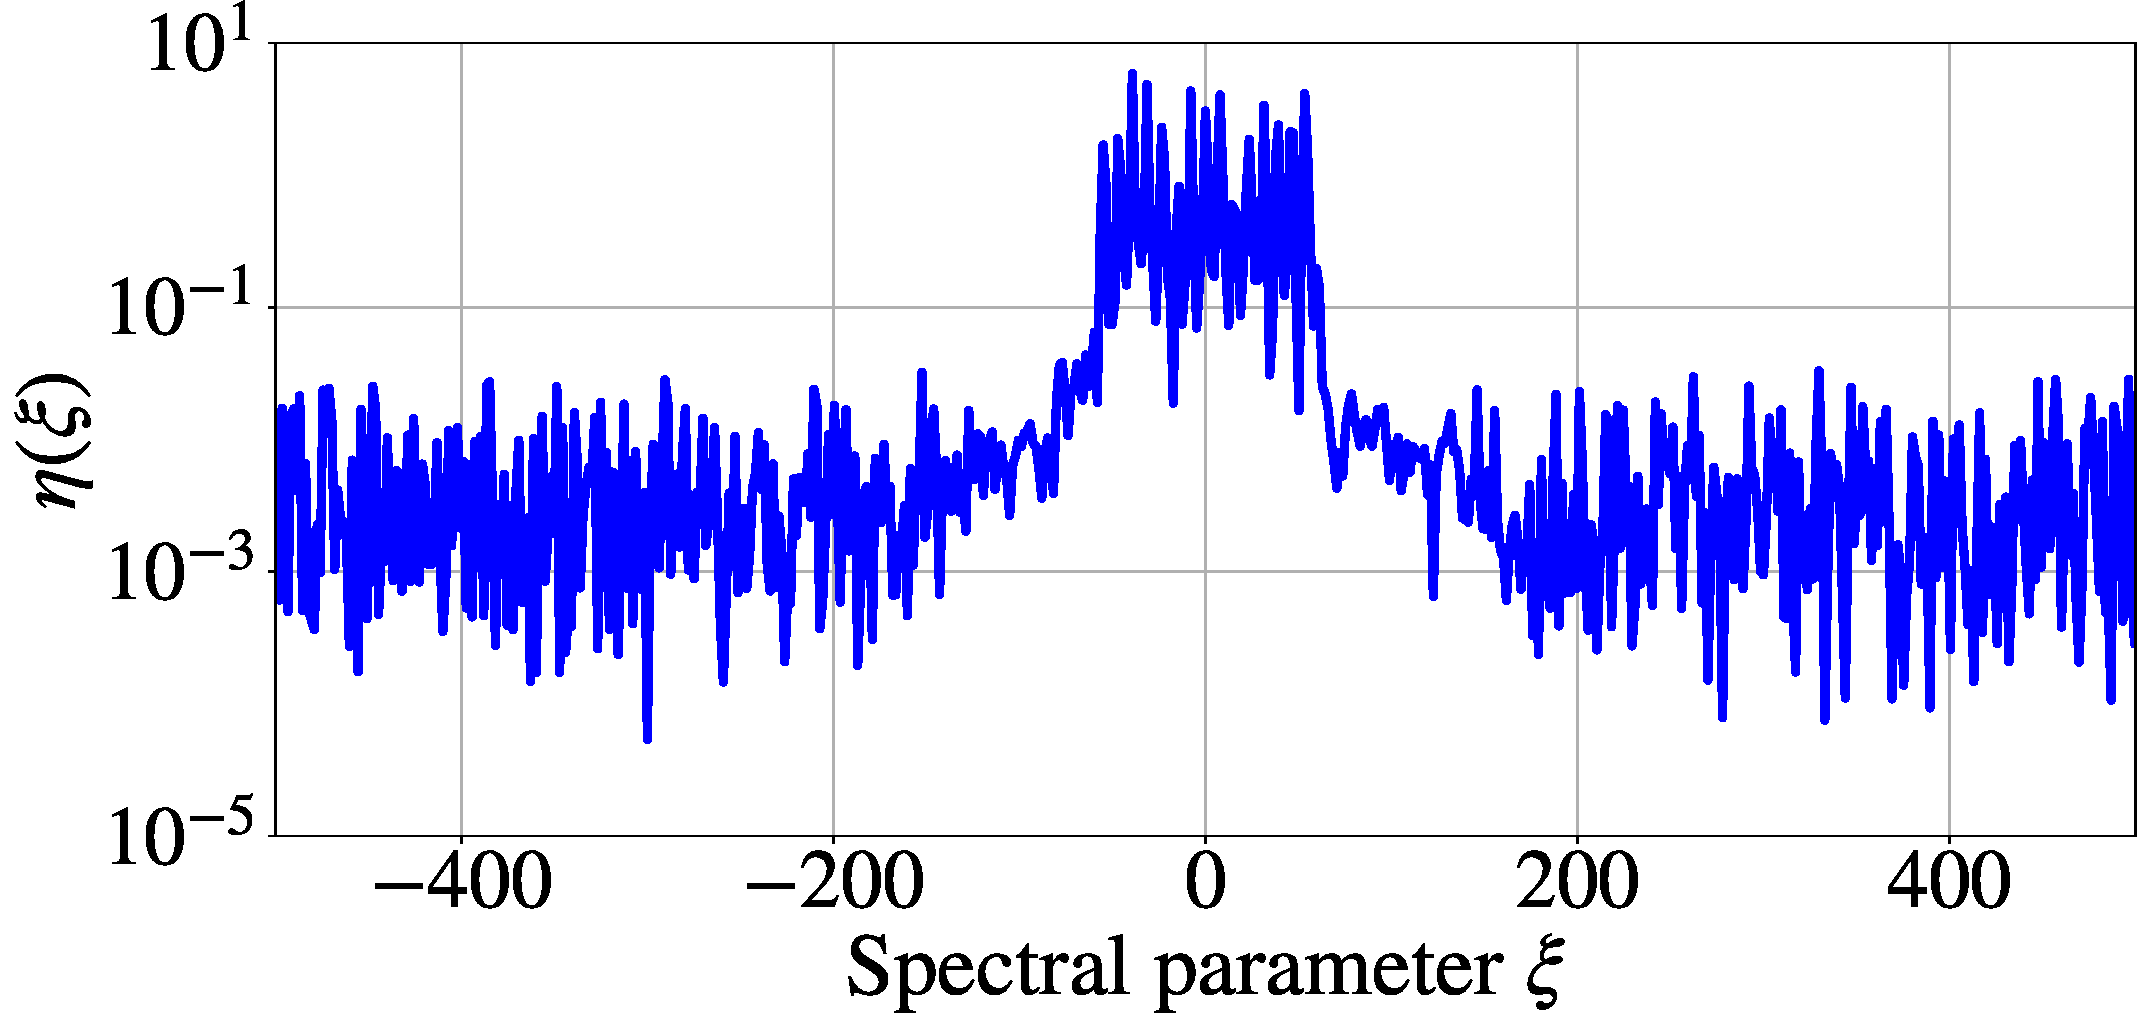
\includegraphics[width=1.\linewidth]{images/nn_nft/scirep_spectrum_diff_wn_example.pdf}
  \center{(f) Difference between $r(\xi)$ calculated using NFT-Net and Conv. \acrshort{nft}}
  % \label{fig:wn_diff}
\end{minipage}


\caption{Panel \textbf{(a)} shows an exemplary amplitude of a original complex WDM signal $q(t)$ versus time. Below (panel \textbf{(c)}) is the amplitude for calculated scattering coefficient $r(\xi)$ associated with the signal from the pane above. The blue line corresponds to the data obtained using the conventional \acrshort{nft} method, the red line corresponds to the NFT-Net result. The difference between the scattering coefficients for signal example calculated by these methods is shown in panel \textbf{(e)}. Pane \textbf{(b)}: the same plot for complex signal $q(t)$ with the addition of Gaussian noise. The \acrshort{snr} value used is 5 dB. Plot \textbf{(d)} shows the result of calculating the continuous spectrum for the noisy signal using the \acrshort{fnft} method (green line) and using the NFT-Net trained at the same noise level (\acrshort{snr} = 5 dB, red line) and original spectrum (for noiseless case, blue line). For NFT-Net trained with noise, pane \textbf{(f)} below shows the difference between the predicted scattering data for the example of noisy signal and the reflection coefficient calculated by conventional \acrshort{nft} for that signal without noise.}
\label{fig:wdm_and_spectrum}
\end{figure}


The results of our comparison for $r(\xi)$ computation using different \acrshort{snr} levels for NFT-Net are presented in Table \ref{tab:nn_with_nft}, and are arranged as follows. The first column of the table identifies the \acrshort{snr} value in dB for the validation signals, i.e. the level of noise for the signals which we analyse. The first row of the table displays the \acrshort{snr} values of noisy signals from the training set, i.e. it shows the noise level of the signals on which the NFT-Net was trained. We notice that the case $\text{SNR}=30$ dB corresponds to almost negligible noise, while for $\text{SNR}=0$ dB our noise energy is equal to that of our signal, which signifies a very intensive noisy corruption. Thus, each column in the table corresponds to the results produced by the \acrshort{nn} trained on the signals with the chosen level of a noisy corruption.
The number in each cell shows the averaged metric value, Eq.~(\ref{eq:metric}), where for the computation of $\{r_{\text{predicted}}(\xi)\}_{i}$ we used the NFT-Net trained on the signals with \acrshort{snr} values shown in the first row and applied to the validation signals having the \acrshort{snr} values given in the first column. The ``Conv. \acrshort{nft}'' column shows the error value for the numerical result of the fast \acrshort{nft} method on the signals with added noise, where the respective \acrshort{snr} is presented, again, in the first column. The value of metric~(\ref{eq:metric}) corresponding to the conventional \acrshort{nft} method applied to noiseless signals is, obviously, zero: the results provided by the conventional \acrshort{nft} without noise are taken as the true ones. 
When the NFT-Net produces a less accurate result compared to the conventional \acrshort{nft} applied to the noisy signal, the cell is marked with grey shadowing; when the NFT-Net outperforms the conventional \acrshort{nft} method, i.e. it successfully purifies our signal from noise, the respective cell is not highlighted (white). 
Whence, the white area size in each table demonstrates how well the NFT-Net retrieves the nonlinear spectrum for noise-corrupted signals.


% Table 6x2 linear
\begin{table}[h!]
\centering
\resizebox{1.\textwidth}{!}
{
\begin{tabular}{ >{\columncolor{White}}p{0.001\linewidth}  >{\columncolor{White}}c | >{\columncolor{White}}c | c c c c c c c c c}

% \begin{tabular}{p{0.001\linewidth} c | c | c c c c c c c c c}
  
  & & & \multicolumn{9}{c}{Training SNR level, dB} \\
  
  & & Conv. NFT & w/o noise & 30 & 25 & 20 & 17 & 13 & 10 & 5 & 0 \\
  \hline
  \rowcolor{LightGray} \cellcolor{White} &
  \cellcolor{White} w/o noise & \cellcolor{White} 0 & 8.39e-4 & 6.52e-3 & 9.43e-3 & 1.26e-2 & 1.61e-2 & 2.38e-2 & 3.59e-2 & 7.43e-2 & 1.42e-1 \\
  
  &
  30 & 6.91e-2 & 5.54e-2 & 9.56e-3 & 1.11e-2 & 1.36e-2 & 1.68e-2 & 2.42e-2 & 3.63e-2 & \cellcolor{LightGray} 7.49e-2 & \cellcolor{LightGray} 1.44e-1 \\

  &
  25 & 1.23e-1 & 9.84e-2 & 1.40e-2 & 1.39e-2 & 1.51e-2 & 1.78e-2 & 2.45e-2 & 3.63e-2 & 7.47e-2 & \cellcolor{LightGray} 1.43e-1 \\

  &
  20 & 2.21e-1 & 1.74e-1 & 2.53e-2 & 2.18e-2 & 1.97e-2 & 2.08e-2 & 2.58e-2 & 3.65e-2 & 7.40e-2 & 1.43e-1 \\

  &
  17 & 3.10e-1 & 2.41e-1 & 3.96e-2 & 3.23e-2 & 2.63e-2 & 2.53e-2 & 2.78e-2 & 3.70e-2 & 7.31e-2 & 1.42e-1 \\

  &
  13 & 4.89e-1 & 3.66e-1 & 7.74e-2 & 6.12e-2 & 4.53e-2 & 3.97e-2 & 3.54e-2 & 3.98e-2 & 7.06e-2 & 1.38e-1 \\

  &
  10 & 6.78e-1 & 4.88e-1 & 1.29e-1 & 1.03e-1 & 7.36e-2 & 6.23e-2 & 5.12e-2 & 4.85e-2 & 6.87e-2 & 1.33e-1 \\

  & 
  5 & 1.16e+0 & 7.26e-1 & 2.73e-1 & 2.31e-1 & 1.72e-1 & 1.43e-1 & 1.15e-1 & 9.93e-2 & 7.98e-2 & 1.17e-1 \\

  \multirow{-9}{*}{\rotatebox[origin=c]{90}{Validation SNR level, dB}}& 
   0 & 2.00e+0 & 9.48e-1 & 4.79e-1 & 4.37e-1 & 3.60e-1 & 3.12e-1 & 2.59e-1 & 2.29e-1 & 1.74e-1 & 1.16e-1 \\

    
\end{tabular}
}
\caption{Comparison of the NFT-Net performance against the conventional NFT in the computation of coefficient $r(\xi)$. The table presents the results for the optimised NFT-Net architecture from Fig.~\ref{fig:nn_architecture}. The values in the cells show the error value (\ref{eq:metric}) for each specific pair of training and validation sets SNR. The gray cells correspond to the cases when the accuracy of the NFT-Net nonlinear spectrum restoration is lower than that of fast NFT, i.e. the NN does not denoise the signal well, while the white cells correspond to the cases when the accuracy of the continuous NF spectrum rendered by the NFT-Net is higher, i.e. the NN effectively denoises the result.}
\label{tab:nn_with_nft}
\end{table}

Table \ref{tab:nn_with_nft} shows the error values for the restoration of $r(\xi)$ coefficient (\ref{eq:nlse_r}) of a noiseless and noisy-perturbed signals (\ref{eq:wdm}), by the NFT-Net architecture given in Fig.~\ref{fig:nn_architecture}. The first row in the table corresponds to the noiseless case. It is always marked with grey, which means that the \acrshort{nn} cannot provide any better results than the benchmark ones rendered by the conventional fast \acrshort{nft} method used to generate the training data. 

However, the values of the error for noise-corrupted signals reveal interesting tendencies. 
It follows from the table that for the low training noise level (up to 10 dB, columns three through nine), the NFT-Net error is typically lowest for the noiseless validation dataset (second row).
Thus, the addition of low noise in the training dataset only degrades the NFT-Net restoration capability, even though this decrease is not significant. This NFT-Net feature can be deemed as the \acrshort{nn}'s being ``confused'' by the weak noise in its training in the nonlinear transformation identification. 
For the most interesting case of high noise, the network works best for samples where the \acrshort{snr} value is the same for the validation and training sets. 
In such cases, the relative error is about 8-12\%, while the error for conventional \acrshort{nft} is at the level of 100-200\%.
Another fact is that with decreasing noise (rows from bottom to top) in the validation set, the error value remains at approximately the same level after the cell corresponding to the same training and validation noise values. 
These results confirm that the presented \acrshort{nn} architecture is capable of performing the desired nonlinear transformation, the \acrshort{nft}, and, in addition, it can also work as an effective denoising element when the noise level becomes non-negligible. 



The examples of original and noise-corrupted signals and the corresponding nonlinear continuous spectra are given in Fig.~\ref{fig:wdm_and_spectrum}, where we used the NFT-Net for the computations. Figures~\ref{fig:wdm_and_spectrum}b and~\ref{fig:wdm_and_spectrum}d show that when the additional noise distorts the signal, the conventional numerical algorithms naturally produce the noise-distorted nonlinear spectra.
Figs.~\ref{fig:wdm_and_spectrum}e and~\ref{fig:wdm_and_spectrum}f show the relative error value $\eta(\xi)$~(\ref{eq:metric}) for the continuous spectrum prediction with NFT-Net for the signal without noise (left) and the signal with noise (right), and the reflection coefficient computed for the original signal by the conventional \acrshort{nft} (marked as ``Conv. \acrshort{nft}'' in the panes' legends). In Figs.~\ref{fig:wdm_and_spectrum}c,~\ref{fig:wdm_and_spectrum}e, the NFT-Net is trained on the dataset without adding noise, and in Figs.~\ref{fig:wdm_and_spectrum}d,~\ref{fig:wdm_and_spectrum}f, the NFT-Net is trained on the dataset with additional noise for \acrshort{snr} = 5 dB. Figs.~\ref{fig:wdm_and_spectrum}c and~\ref{fig:wdm_and_spectrum}d show that in the presence of noise, the fast \acrshort{nft} results begin to deviate noticeably from the original (noiseless) values, while the NFT-Net tends to denoise the resulting nonlinear spectrum.








\subsection{NFT-Net performance for the restoration of \acrshort{nf} coefficient $b(\xi)$ attributed to noisy signals}
In addition to the coefficient $r$, from the optical communications perspective it is instructive and important to check how the proposed architecture would work to predict the \acrshort{nf} coefficient $b$, Eq.~(\ref{eq:nlse_ab}). We note that the optical transmission method coined b-modulation \cite{w17,wsh20,svp20}, where we operate with the modulation of the b-coefficient, has proven to be the most efficacious technique among different \acrshort{nfdm} methods proposed \cite{yal19,yla19}. Moreover, for the practical case when our signal has a finite extent, the continuous part of the \acrshort{nf} spectrum can be completely described by the b-coefficient only, because the second \acrshort{nf} coefficient $a(\xi)$ can be calculated from $b(\xi)$ profile, see Eq.~(\ref{a-fin}) in Methods. Our goal here is to demonstrate that the same NFT-Net structures can be used for the both $r(\xi)$ and $b(\xi)$ computation, when the \acrshort{nn} is trained on the respective dataset. As the loss function, we now use the \acrshort{mse} build on the b-coefficient samples, and the \acrshort{mse} is also used as our quality metric in the respective tables:
\begin{equation}
    \eta_b = \frac{1}{S} \, \sum_{i = 1}^{S} \langle \eta_{b,i}(\xi) \rangle_{\xi}, 
    \qquad 
    \eta_{b,i}(\xi) = \frac{|\{b_\text{predicted}(\xi)\}_i - \{b_\text{actual}(\xi)\}_i| }{\langle |\{b_\text{actual}(\xi)\}_i| \rangle_{\xi}}.
    \label{eq:b_metric}
\end{equation}
The notations are the same as we used in~(\ref{eq:metric}): the labels ``predicted'' and ``actual'' correspond, respectively, to the result of the NFT-Net applied to noisy signals and the result produced by the conventional \acrshort{nft} routine applied to noiseless signals.

We carried out the analysis of the NFT-Net performance for the restoration of b-coefficient using the same approach as we did in the previous subsection for $r(\xi)$. Our results for noise pulses with the different level of noise are summarised in Table~\ref{tab:nn_with_nft_b}. 
We checked that the NFT-Net configurations when applied to the computation and denoising of $b(\xi)$ revealed the same tendencies for the quality of restoration as we observed in the previous subsection devoted to the reflection coefficient $r(\xi)$.
\begin{table}[h!]
\centering
\resizebox{1.\textwidth}{!}
{
\begin{tabular}{ >{\columncolor{White}}p{0.001\linewidth}  >{\columncolor{White}}c | >{\columncolor{White}}c | c c c c c c c c c}
  
  & & & \multicolumn{9}{c}{Training SNR level, dB} \\
  
  & & Conv. NFT & w/o noise & 30 & 25 & 20 & 17 & 13 & 10 & 5 & 0 \\
  \hline
  \rowcolor{LightGray} \cellcolor{White} &
  \cellcolor{White} w/o noise & \cellcolor{White} 0 & 7.12e-3 & 5.37e-3 & 5.87e-3 & 6.49e-3 & 8.69e-3 & 1.07e-2 & 1.20e-2 & 1.58e-2 & 1.77e-2 \\
  
  & 30 & 1.15e-1 & 5.83e-2 & 6.73e-3 & 6.69e-3 & 7.16e-3 & 8.95e-3 & 1.08e-2 & 1.20e-2 & 1.58e-2 & 1.77e-2 \\

  & 25 & 2.05e-1 & 1.02e-1 & 1.02e-2 & 8.70e-3 & 8.48e-3 & 9.54e-3 & 1.09e-2 & 1.21e-2 & 1.58e-2 & 1.77e-2 \\

  & 20 & 3.64e-1 & 1.75e-1 & 2.13e-2 & 1.51e-2 & 1.18e-2 & 1.12e-2 & 1.14e-2 & 1.23e-2 & 1.59e-2 & 1.78e-2 \\

  & 17 & 5.14e-1 & 2.38e-1 & 3.66e-2 & 2.41e-2 & 1.59e-2 & 1.33e-2 & 1.21e-2 & 1.26e-2 & 1.60e-2 & 1.78e-2 \\

  & 13 & 8.14e-1 & 3.44e-1 & 7.73e-2 & 4.94e-2 & 2.64e-2 & 1.88e-2 & 1.39e-2 & 1.36e-2 & 1.63e-2 & 1.80e-2 \\

  & 10 & 1.15e+0 & 4.41e-1 & 1.31e-1 & 8.58e-2 & 4.21e-2 & 2.70e-2 & 1.67e-2 & 1.51e-2 & 1.69e-2 & 1.84e-2 \\

  & 5 & 2.04e+0 & 6.22e-1 & 2.70e-1 & 1.96e-1 & 9.95e-2 & 5.91e-2 & 2.81e-2 & 2.18e-2 & 1.95e-2 & 1.99e-2 \\

  \multirow{-9}{*}{\rotatebox[origin=c]{90}{Validation SNR level, dB}} & 0 & 3.60e+0 & 7.98e-1 & 4.54e-1 & 3.68e-1 & 2.24e-1 & 1.42e-1 & 6.34e-2 & 4.43e-2 & 2.93e-2 & 2.43e-2 \\

    
\end{tabular}
}
\caption{Comparison of the NFT-Net performance against the fast conventional NFT in the computation of coefficient $b(\xi)$. The table presents the results for the NFT-Net architecture from Fig.~\ref{fig:nn_architecture}. The values in the cells show the error value (\ref{eq:b_metric}) for each specific pair of training and validation sets SNR. The grey cells correspond to the cases when the accuracy of the NFT-Net nonlinear spectrum restoration is lower than that of fast NFT, i.e. the NN does not denoise the signal well, while the white cells correspond to the cases when the accuracy of the continuous NF spectrum rendered by the NFT-Net is higher, i.e. the NN effectively denoises the signal.}
\label{tab:nn_with_nft_b}
\end{table}
A similar situation as was observed for coefficient $r(\xi)$, remains in this case. The error is minimal for a noiseless validation set. However, this trend now continues for high noise levels.
A similar tendency is observed all over the results: the values above the diagonal vary slightly.
The additional observations when dealing the b-coefficient are as follows. An interesting difference from the case relevant to $r(\xi)$, is that the metric value~(\ref{eq:b_metric}) in the case of predicting $b(\xi)$ is less, and the grey-shadowed region in Table \ref{tab:nn_with_nft} is larger compared to what we see in Table \ref{tab:nn_with_nft_b} for the b-coefficient.
From the results, it is clear that the prediction accuracy is higher for the b-coefficient. 
It means that our \acrshort{nn} generally works more accurately for the restoration of coefficient $b(\xi)$ than for $r(\xi)$. This result can be expected, as the noise-perturbed $r(\xi)$ contains the noisy contributions from both $a(\xi)$ and $b(\xi)$, while the b-coefficient involves only its noisy contribution, and thus gets corrupted less. So in the latter case, the \acrshort{nn} has to clean off less noise.

Figure~\ref{fig:quality_r_b} summarizes the above and shows the calculation errors~(\ref{eq:metric}) and~(\ref{eq:b_metric})  for NFT-Net architecture. The plot actually visualises the values and tendencies from Tables \ref{tab:nn_with_nft} and \ref{tab:nn_with_nft_b}. For both $r(\xi)$ and $b(\xi)$ coefficients, the \acrshort{nn} outperforms the fast \acrshort{nft} results when the NFT-Net gets trained on the data with additional noise. 


\begin{figure}[tp]
\centering
\begin{minipage}{.49\textwidth}
  \centering
  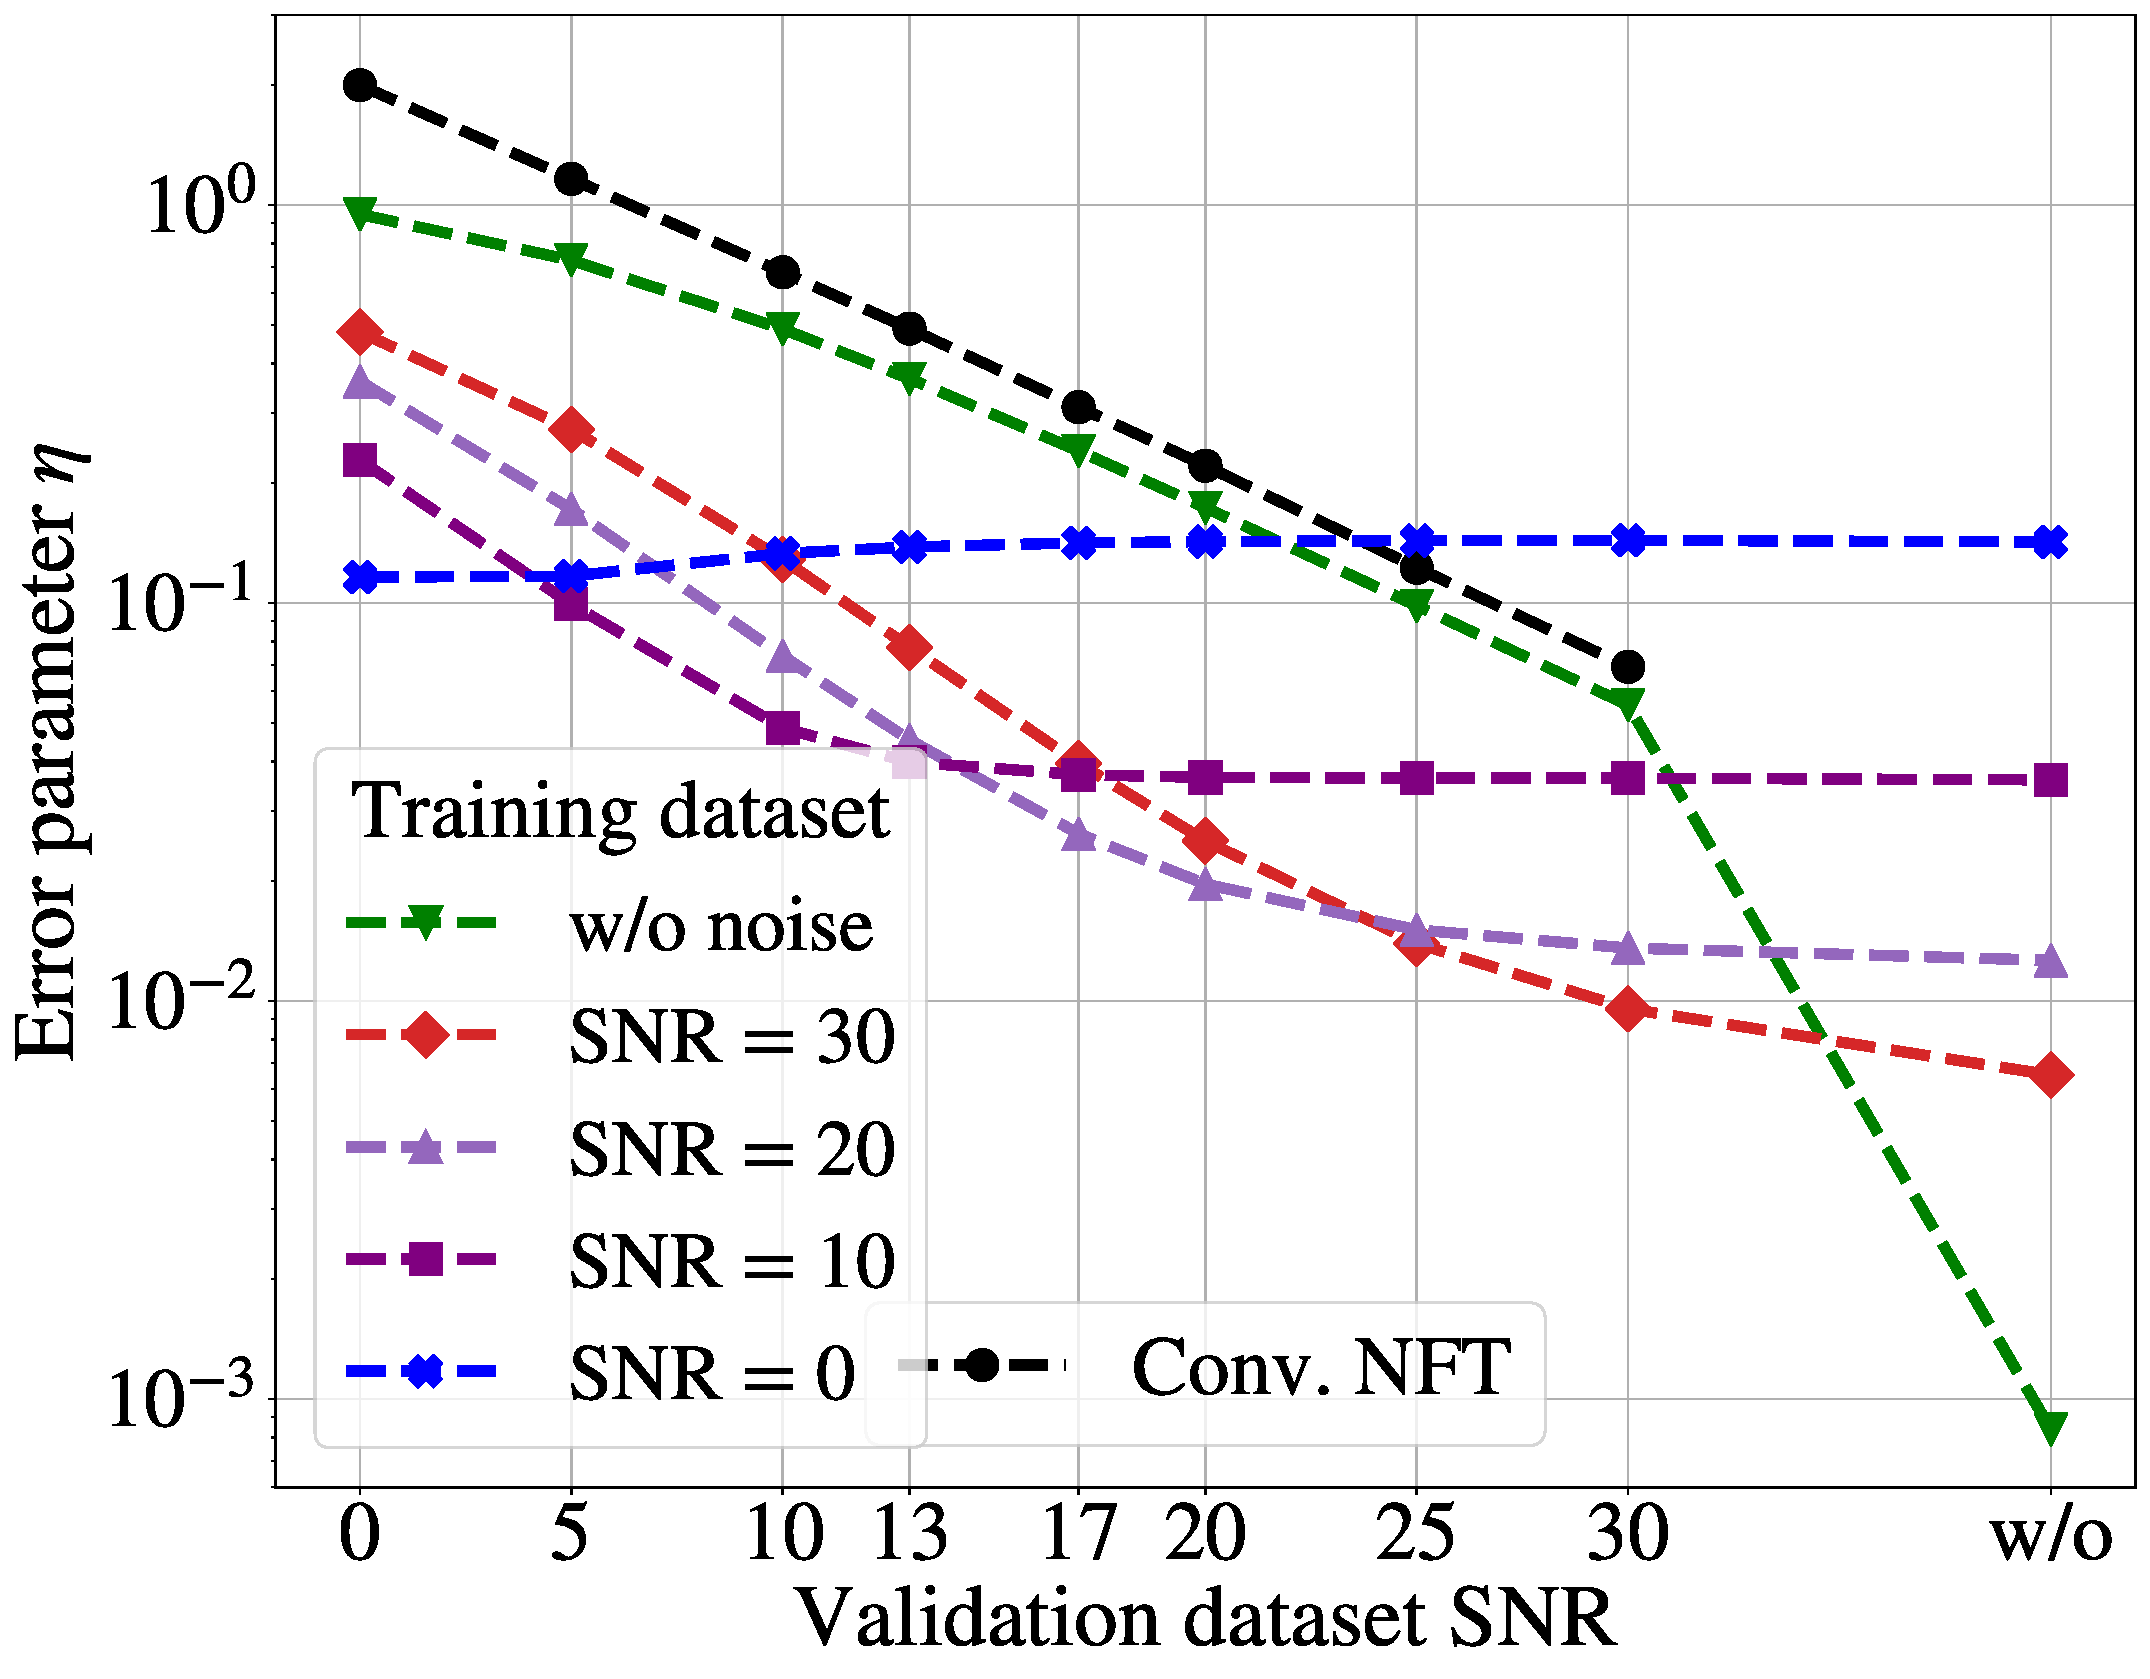
\includegraphics[width=1.\linewidth]{images/nn_nft/scirep_nft_r_metric.pdf}
  % \caption{}
  % \label{fig:quality_r}
\end{minipage}%
\begin{minipage}{.49\textwidth}
  \centering
  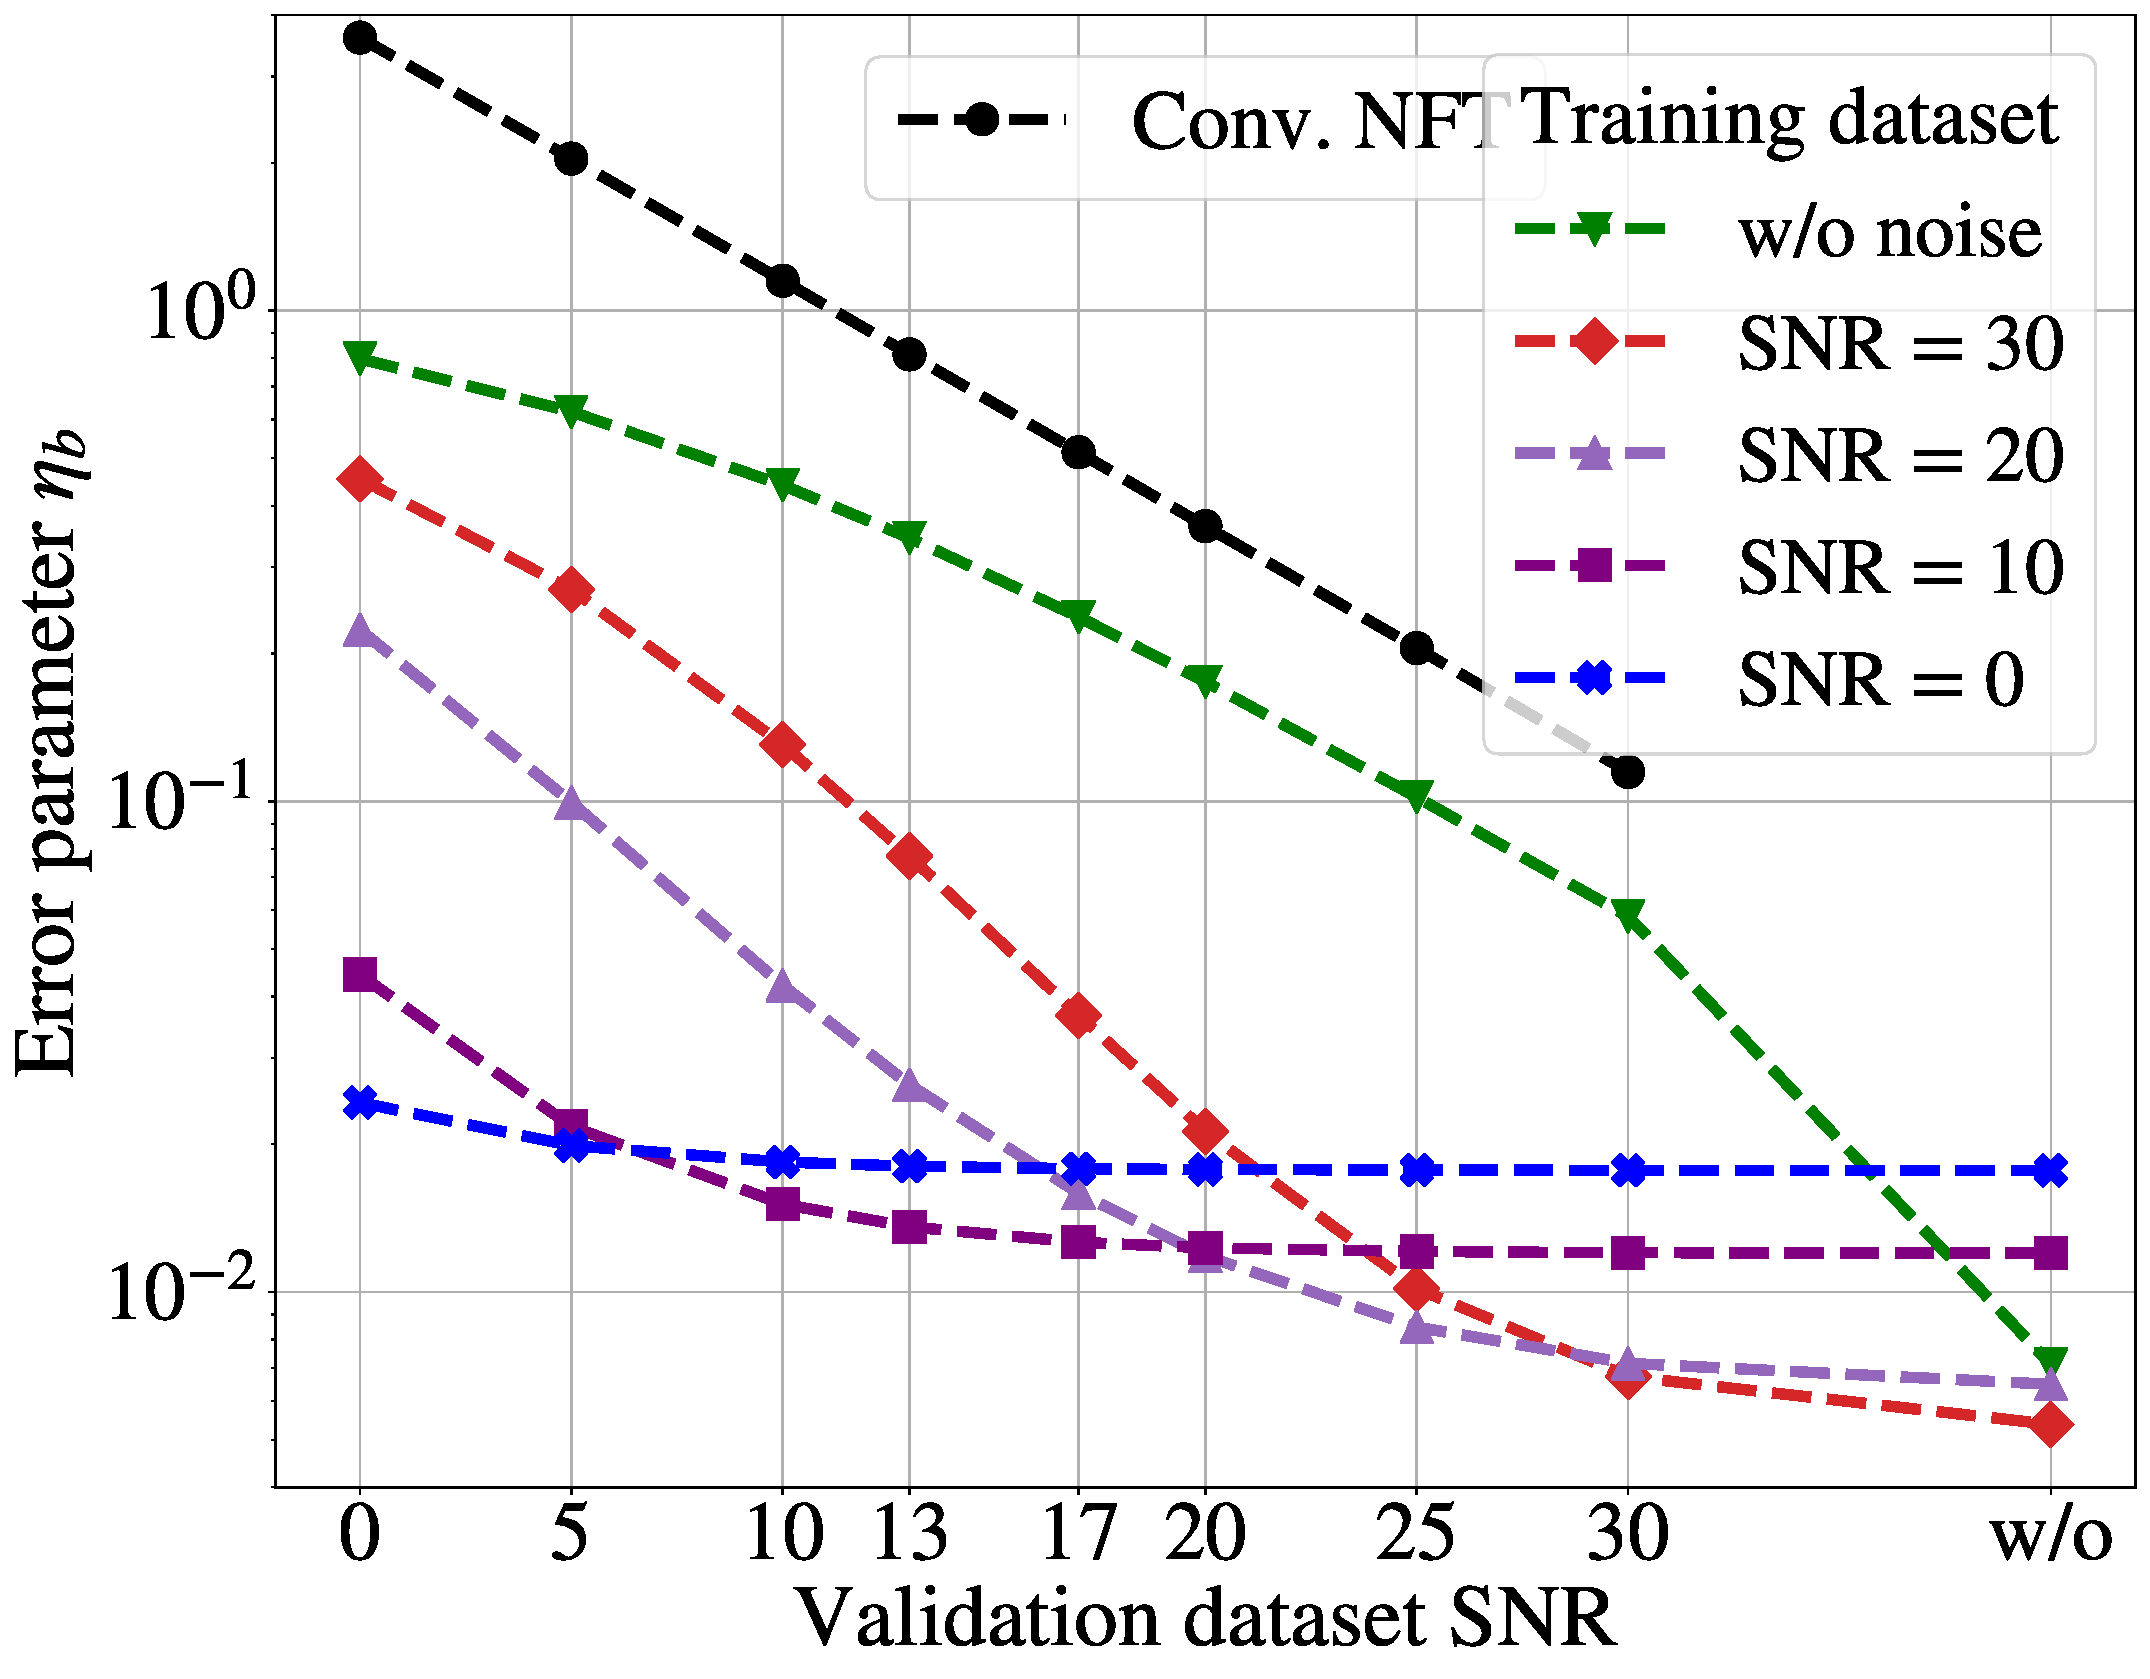
\includegraphics[width=1.\linewidth]{images/nn_nft/scirep_nft_b_metric.pdf}
  % \caption{}
  % \label{fig:quality_b}
\end{minipage}
\caption{\textbf{(a)} The dependence of the error parameter $\eta$~(\ref{eq:metric}) for coefficient $r(\xi)$ on the \acrshort{snr} value of the validation dataset for fast conventional \acrshort{nft} and NFT-Net trained at different noise levels. \textbf{(b)} The same for the error parameter $\eta_b$~(\ref{eq:b_metric}) for coefficient $b(\xi)$. The black line represents the error value for fast \acrshort{nft} applied to noisy signals, and the points below this line refer to the cases when the NFT-Net outperforms conventional computations. Other lines show  the value of the error in calculating the continuous spectrum using NFT-Net, trained with different noise levels: green -- without additional noise, red -- with additional noise with \acrshort{snr} = 30 dB, violet -- at \acrshort{snr} = 20 dB purple -- at \acrshort{snr} = 10 dB, blue -- at \acrshort{snr} = 0 dB.}
\label{fig:quality_r_b}
\end{figure}